\documentclass[a4paper,titlepage,12pt,twoside]{report}
\usepackage[dvipdfmx]{graphicx, xcolor} 
\usepackage{here}
\usepackage{longtable}
\usepackage{makeidx}
\usepackage{amsmath}
\usepackage{amssymb}
\usepackage{multicol}
\usepackage{epsfig}
\usepackage{amsfonts}
\usepackage{multirow}
\usepackage{slashbox}
\usepackage{url}
\usepackage[subrefformat=parens]{subcaption}
\usepackage{bm}
\usepackage{scalefnt}
\usepackage{mathptmx}
\newcommand{\argmin}{\mathop{\rm arg~min}\limits}
\renewcommand{\bibname}{Reference}

%
% 余白の調整 (A4用紙は595ptx842pt)
% 左側の余白
\setlength{\oddsidemargin}{30pt}
% 偶数の左余白
\setlength{\evensidemargin}{30pt}
% 本文テキスト全体の幅
\setlength{\textwidth}{430pt}
% 上側の余白
\setlength{\topmargin}{20pt}
% ヘッダの高さ
\setlength{\headheight}{0pt}
% ヘッダと本文テキストとの間の余白
\setlength{\headsep}{0pt}
% 本文テキスト全体の高さ
\setlength{\textheight}{670pt}

\title{
  \fontsize{23.5pt}{23.5pt} \selectfont{
  Low-Light Image Enhancement\\
  via Mixture L2-LP Variational Retinex Model\\
  with Adaptive Texture Map}
}

%\title{
%  \huge{
%  Low-Light Image Enhancement\\
%  via Mixture L2-LP Variational Retinex Model\\
%  with Adaptive Texture Map}
%}

\author{
  \large{Thesis Supervisor}\\
  \large{Prof.\ Youji Iiguni}\\[1cm]
  \large{Kazuki Kurihara}\\[1cm]
  \large{Division of Systems Science and Applied Informatics}\\
  \large{Department of Systems Innovation}\\
  \large{Graduate School of Engineering Science}\\
  \large{Osaka University}
}
\date{January 28, 2020}

%%%%%%%%%%%%%%%%%%%% 表紙 %%%%%%%%%%%%%%%%%%%%
\begin{document}
\maketitle
\pagestyle{empty}
\cleardoublepage

%%%%%%%%%%%%%%%%%%%% 概要 %%%%%%%%%%%%%%%%%%%%
\pagestyle{plain}
\setcounter{page}{1}  % ページ番号を1に設定
\pagenumbering{roman}
%----Abstruct---- %
\begin{center}
\section*{Abstract}
\end{center}
The methods of low-light image enhancement have been paid attention to with the wide spread of computer vision applications used in outdoors. Many methods have used cost functions which are based on Retinex theory that decomposes an observed image into reflectance and illumination. However, the enhanced image causes negative effects such as halo artifacts, noise amplification, and over-enhancement when the methods can not sufficiently consider the characteristics of reflectance and illumination. Thus, in order to alleviate such effects, we incorporate constraint terms which further consider the characteristics of reflectance and illumination with a cost function. In addition, we develop an adaptive texture map as a weight of the constraint term on reflectance, which is used to tune noise reduction rate according to brightness of an observed image. Moreover, the adaptive texture map contributes to reveal fine textures detail in the estimated reflectance. Both qualitative and quantitative evaluations show that the proposed method can sufficiently enhance low-light images while suppressing halo artifacts, noise amplification, and over-enhancement.

%%%%%%%%%%%%%%%%%%%% 目次 %%%%%%%%%%%%%%%%%%%%
\cleardoublepage
\setcounter{tocdepth}{1}
\tableofcontents 
%\newpage
\mbox{}
\cleardoublepage

%%%%%%%%%%%%%%%%%%%% Documenet %%%%%%%%%%%%%%%%%%%%
\setcounter{page}{1}
\pagenumbering{arabic}
%%%%%%%%%%%%%%%%%%%% Introduction %%%%%%%%%%%%%%%%%%%%
%----導入部分---- %
\chapter{Introduction}
\label{sec:intro}
 Images captured under low light conditions suffer from poor visibility, low contrast, and unexpected noise. Consequently, low-light images prevent human from extracting hidden meaningful information. Moreover, such degradation affect vision techniques, including consumer digital cameras, mobile phones and video surveillance systems, which can be often used in outdoors. Therefore, the methods of low-light image enhancement, including histogram equalization (HE) algorithms \cite{he1} - \cite{he3}, dehaze-based algorithms \cite{haze1}, \cite{haze2}, and Retinex-based algorithms\cite{ssr} - \cite{rrm} have been proposed to deal with above problems. \par
%----Histogram Equalization Method---- %
HE algorithms are probably the most intuitive and simplest way to improve image contrast. The operation stretches the dynamic range of intensity level of an observed image. As a result, the methods tend to result in over-enhancement. In addition, the methods can not consider the intensive noise hidden under dark regions in low light images. Therefore, the methods lead to noise amplification after contrast enhancement.\par
%----Dehazing Method---- %
Some methods \cite{haze1}, \cite{haze2} noticed that the inverted low-light images look like haze images. According to this observation, the methods attempted to deal with low-light images. Although the methods can obtain reasonable results, they do not provide a sufficient physical explanation for the basic model.
%----Retinex Model---- %
Many methods that focus on Retinex theory, which is a color perception model based on human visual system, have been proposed for low-light image enhancement. According to the basic assumption of Retinex theory \cite{retinex}, an observed image can be decomposed into two parts: reflectance and illumination. Early attempts in this theory, such as Single-Scale Retinex (SSR) \cite{ssr} and Multi-Scale Retinex (MSR) \cite{msr}, treat reflectance as the enhancement result. However, the methods cause over-enhancement and generate unrealistic result. This problem is mainly caused by the logarithmic operation when enhancing a low-light image. To overcome this problem, Fu proposed a simultaneous reflectance and illumination estimation (SRIE) \cite{srie} and a weighted variation model (WVM) \cite{wvm}. The methods demonstrated that the linear domain model is better than the log-transformed domain in preserving naturalness. These methods have good performances in the enhancement, but they still have the problem that noise is quite observable in the results, especially when an observed image has much noise in dark regions. Cai $et$ $al$. \cite{jiep} proposed a Joint intrinsic-extrinsic Prior (JieP) model for Retinex decomposition by considering the properties of 3D objects. The method can significantly distinguish between texture and structure regions and estimate illumination while keeping the structure information. However, the method generates noise amplification in dark regions, since the method can not sufficiently consider the constraint term on reflectance. Li presented a robust Retinex model (RRM) \cite{rrm} by adding a noise term to the cost function in order to deal with noise amplification due to the estimation errors. RRM effectively suppresses noise amplification, but the method has difficulty balancing piece-wise smoothed illumination and details of reflectance. Many above methods adopt a $L_{1}$ norm to the constraint term on reflectance, but the tiny details of the estimated reflectance are susceptible to be damaged. Moreover, by adopting a $L_{2}$ norm to the constraint term on illumination, the estimated illumination is over-smoothed without keeping the structure information. \par
In this paper, we propose a new cost function that further considers the characteristics of both reflectance and illumination. We adopt $L_{2}$ and $L_{p}$ norms to the constraint terms on reflectance and illumination in order to preserve fine textures detail as much as possible, and smooth illumination as as much as possible while keeping the structure information. Moreover, we introduce an adaptive texture map into a weight of the constraint term on reflectance. The adaptive texture map is used to tune a noise reduction rate according to brightness of an observed image. In addition, the adaptive texture map contributes to reveal fine textures detail in the estimated reflectance. Finally, we show that the proposed method outperforms the state-of-the-art methods in both qualitative and quantitative evaluations.\par
\cleardoublepage
%%%%%%%%%%%%%%%%%%%% Related Work %%%%%%%%%%%%%%%%%%%%
\chapter{Related Work}
\label{sec:related}

%----Retinex理論の説明---- %
\section{Retinex Theory} \label{sec:retinex}
The Retinex theory \cite{retinex} is a color perception model based on human visual system. The model decomposes an observed image into the reflectance and illumination as follows:
\begin{equation}
S = R \circ I,\label{eq:retinex}
\end{equation}
where $S$ is an observed image, $R$ and $I$ represent the reflectance and the illumination, respectively. The operator $\circ$ denotes the element-wise multiplication. As shown in Fig. \ref{fig:retinex}, the reflectance represents the intrinsic characteristics of the object and contains rich textures detail. On the contrary, the illumination represents the extrinsic property and contains the structure information with texture-less.

%----Retinex理論のイメージ図---- %
\begin{figure}[tb]
	\begin{minipage}[b]{0.32\hsize}
		\centering
		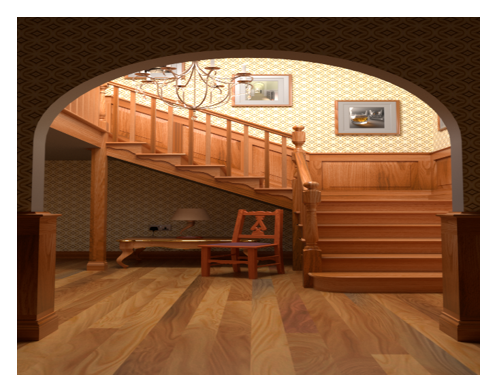
\includegraphics[height=0.75\hsize]{images/retinex/input.eps}
		\subcaption{Observed image $S$} \label{fig:reinex/input}
	\end{minipage}
	\begin{minipage}[b]{0.32\hsize}
		\centering
		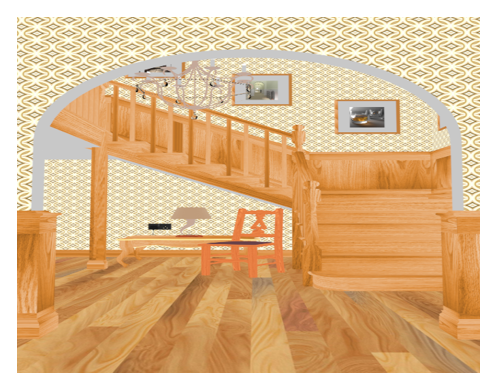
\includegraphics[height=0.75\hsize]{images/retinex/reflectance.eps}
		\subcaption{Reflectance $R$} \label{fig:retinex/reflectance}
	\end{minipage}
	\begin{minipage}[b]{0.32\hsize}
		\centering
		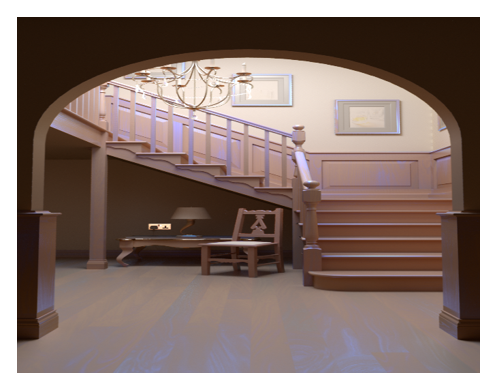
\includegraphics[height=0.75\hsize]{images/retinex/illumination.eps}
		\subcaption{Illumination $I$} \label{fig:retinex/illumination}
	\end{minipage}
\caption{The images represent Retinex theory \cite{arpr}.}
\label{fig:retinex}
\end{figure}

The conventional Retinex-based enhancement methods such as \cite{ssr}, \cite{msr} are defined as
\begin{equation}
\log{R} = \log{S} - \log{[G \ast S]}, \label{eq:log_retinex}
\end{equation}
where $\ast$ represents the convolution operator, $G$ is the Gaussian low-pass filter. This method assumes that illumination can be estimated by the Gaussian low-pass filtered version of an observed image. Moreover, the reflectance is computed by subtracting the estimated illumination from an observed image. However, this method generates the halo effect around the edges of object according to the size of the Gaussian low-pass filter. In addition, as shown in Fig. \ref{fig:msr}, this method cause over-enhancement and much noise in the estimated reflectance. 

\begin{figure}[tb]
\begin{minipage}[b]{0.5\hsize}
		\centering
		\includegraphics[height=0.6\hsize]{images/msr/input.eps}
		\subcaption{Observed image $S$} \label{fig:msr/input}
	\end{minipage}
	\begin{minipage}[b]{0.5\hsize}
		\centering
		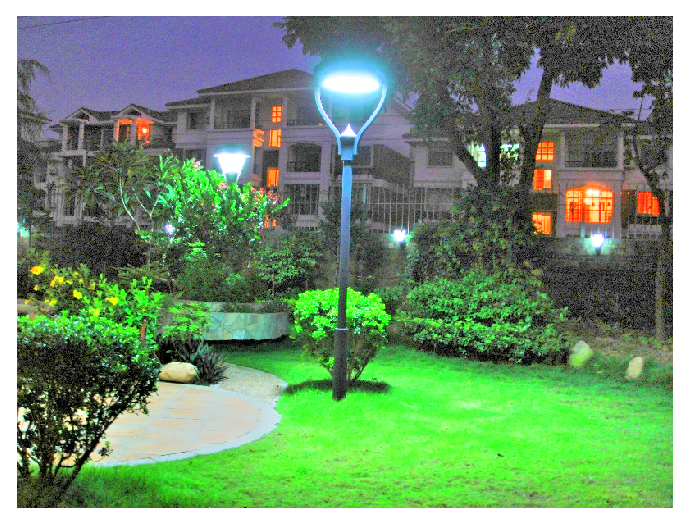
\includegraphics[height=0.6\hsize]{images/msr/reflectance.eps}
		\subcaption{Reflectance $R$} \label{fig:msr/reflectance}
	\end{minipage}
\caption{The images represent the result of the conventional Retinex-based enhancement method \cite{msr}.}
\label{fig:msr}
\end{figure}

%----Variational Retinex Modelの説明---- %
\section{Variational Retinex Model} \label{sec:variational_retinex}
Various researches have proposed energy minimization problems based on Retinex in order to efficiently estimate reflectance and illumination. These methods estimate reflectance and illumination by setting the constraint terms which consider the characteristics for their component. Thus, it is important for these methods to adopt the appropriate constraints for their component in order to deal with halo effect, over-enhancement, and noise amplification. These methods usually adopt the $L_{1}$ and $L_{2}$ norm regularization to the constraint terms. To give an example, Fu \cite{srie} proposed the minimizing optimization problem derived as
\begin{equation}
\begin{split}
& E(I, R) = \argmin_{R, I} \|R \circ I - S\|_{2}^{2} + \alpha\|\nabla{I}\|_{2}^{2} + \beta\|\nabla{R}\|_{1} + \gamma\|I - I_{0}\|_{2}^{2} \\
& s.t. \ \ S \leqq I, \label{eq:srie_equation}
\end{split}
\end{equation}
where $\alpha$, $\beta$, $\gamma$ are three positive parameters, and $I_{0}$ is the enhanced illumination using gamma correction.
The first term $\|R \circ I - S\|_{2}^{2}$, which corresponds to L2 data fidelity, is to minimize the distance between the estimated ($R\circ{I}$) and an observed image $S$. The second term $\|\nabla{I}\|_{2}^{2} $ enforces spatially smoothness on the illumination $I$. The third term $\|\nabla{R}\|_{1}$, which corresponds to TV reflectance sparsity, enforces piece-wise continuous on the reflectance $R$. The last term $\|I-I_{0}\|_{2}^{2}$, which penalizes the brightness of illumination component, is used to avoid a scaling problem. \par
This method demonstrated the linear domain model is better than the log-transformed domain model in preserving naturalness. As shown in Fig. \ref{fig:variational/srie}, this method employs the third term which minimizes the difference between $I$ and $I_{0}$ for the sake of suppression of over-enhancement in the estimated reflectance. Moreover, this method can suppress noise amplification due to the $L_{1}$ norm regularization on the reflectance in the estimated reflectance.

%----SRIEの図---- %
\begin{figure}[tb]
	\begin{minipage}[b]{0.5\hsize}
		\centering
		\includegraphics[width=62.5mm]{images/variational/input.eps}
		\subcaption{Observed image $S$} \label{fig:variational/input}
	\end{minipage}
	\begin{minipage}[b]{0.5\hsize}
		\centering
		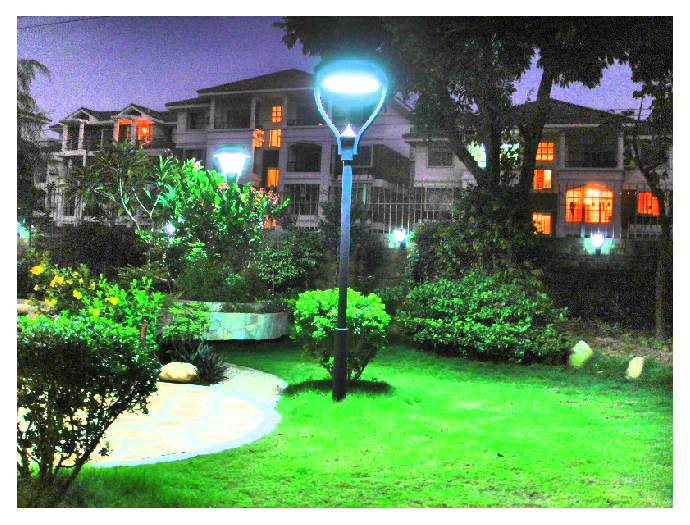
\includegraphics[width=62.5mm]{images/variational/reflectance.eps}
		\subcaption{Reflectance $R$} \label{fig:variational/reflectance}
	\end{minipage}
	\begin{minipage}[b]{0.5\hsize}
		\centering
		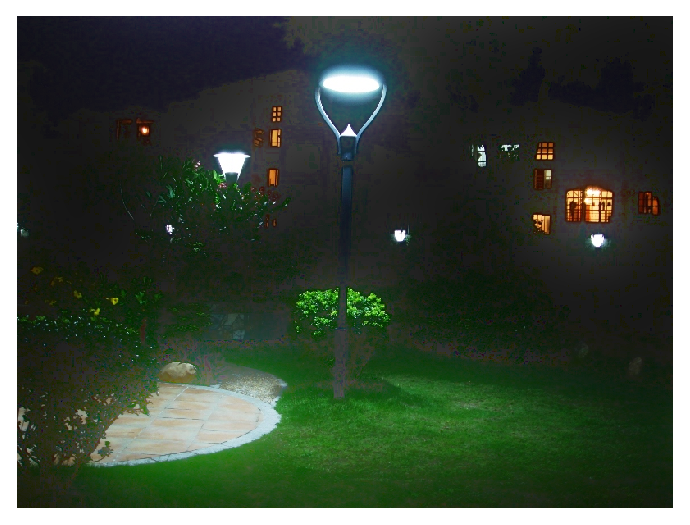
\includegraphics[width=62.5mm]{images/variational/illumination.eps}
		\subcaption{Illumination $I$} \label{fig:variational/illumination}
	\end{minipage}
	\begin{minipage}[b]{0.5\hsize}
		\centering
		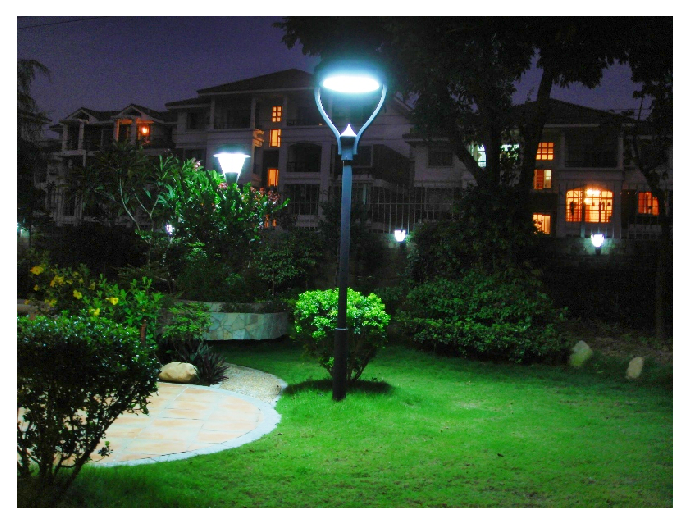
\includegraphics[width=62.5mm]{images/variational/output.eps}
		\subcaption{Enhanced image $\hat{S}$} \label{fig:variational/output}
	\end{minipage}
	\caption{The images represent the result of SRIE \cite{srie}.}
	\label{fig:variational/srie}
\end{figure}

%----Edge Preserving Filterの説明---- %
\section{Local Variation Deviation} \label{sec:lvd}
In this section, the review centers on the edge/structure preserving image smoothing and the joint intrinsic-extrinsic prior model (JieP), which proposed by Cai \cite{jiep} and adopted the image smoothing function as the constraint term on the illumination in (\ref{eq:srie_equation}). 
%The illumination is piece-wisely smooth component, which can be decomposed by a edge preserving smoothing.
\par
In statics, the standard deviation represents a measure to quantify the consistency of a set of data. The local variation deviation (LVD) is used to identify different type of the variation with its statistical property. By using the feature in the image analysis, the local variation deviation can surprisingly distinguish between texture and structure, since texture component has the feature of weak correlation and structure component has the feature of strong correlation. \par
The $\mathcal{R}_{d}$ denotes the relative LVD extracted from $I$:

\begin{equation}
\mathcal{R}_{d} = \left |\frac{\nabla_{d}{I}}{\frac{1}{\Omega}\Sigma_{\Omega}\nabla_{d}{I}+\epsilon} \right| ,
\label{eq:lvd}
\end{equation} 
where $\nabla_{d}$ is the horizontal/vertical ($d \in {h, v}$) gradient operator, $\Omega$ is the local patch size $(r \times r)$, and $\epsilon$ is a small number to avoid division by zero. 
The edge/structure preserving smoothing property of the LVD can be explained intuitively as following.
(In the following, the variable of the mean local variation means $\bar{\nabla{I}}= \frac{1}{|\Omega|} \Sigma_{\Omega}\nabla{I}$):

\begin{itemize}
\item Case1: \textbf{Flat.} If the value of the patch $I$ is almost constant, $\nabla{I} \approx 0$ and $\bar{\nabla{I}} \approx 0$ $\rightarrow$ $\bar{\mathcal{R}} \approx 0$. 
\item Case2: \textbf{Texture.} If the value of the patch $I$ changes frequently, $\nabla{I} $ varies more rapidly than $\bar{\nabla{I}}$ $\rightarrow$ $\bar{\mathcal{R}}$ $\gg 1$.
\item Case3: \textbf{Structure.} If the value of the patch $I$ changes in accordance with structure, the deviation of $\nabla{I}$ fluctuates small $\rightarrow$ $\bar{\mathcal{R}}$ $\approx 1$.
\end{itemize}
To quantitatively analyze the effectiveness of the distinction of the LVD measure, Fig.\ref{fig:jiep/analysis} shows the average value of the LVD in the local patches. The blue regions represent textures and the green regions represent structures. As shown in Fig.\ref{fig:jiep/analysis}, there is a clear difference between texture and structure regions.

\begin{figure}[tb]
	\centering
	\includegraphics[width=0.8\hsize]{images/jiep/analysis/analysis.eps}
	\caption{The images represent local variation deviation for different patches. $\bar{\mathcal{R}}$ is the average of variation deviation in the local patches. The local variation deviation surprisingly distinguish textures (blue regions) and structures (green regions).
	} \label{fig:jiep/analysis}
\end{figure}

Thanks to the performance of the LVD, Cai replaced the constraint term on the illumination with the LVD on the illumination in the minimization optimization problem as following:
\begin{equation}
 E(I, R) = \argmin_{R, I} \|R \circ I - S\|_{2}^{2} + \alpha{\left \|\frac{\nabla{I}}{\frac{1}{\Omega}\Sigma_{\Omega}\nabla{I} + \epsilon} \right\|_{1}} + \beta{\|\nabla{R}\|_{1}} + \gamma{\|I - B\|_{2}^{2}}, \label{eq:jiep}
\end{equation}
where $\alpha$, $\beta$, $\gamma$ are three positive parameters and $B$ ($B = max_{\Omega}(max_{c \in \{r, g, b\}}S_{c})$) represents the bright channel prior (BCP) of an observed image $S$. As shown in Fig.\ref{fig:jiep/example}, the estimated illumination removes texture component while preserving the structure information. Thus, in the estimated reflectance, JieP significantly suppresses the awareness of halo effect along with edge regions. Moreover, more textures detail reveal in the estimated reflectance.

%----JiePの図---- %
\begin{figure}[tb]
	\begin{minipage}[b]{0.5\hsize}
		\centering
		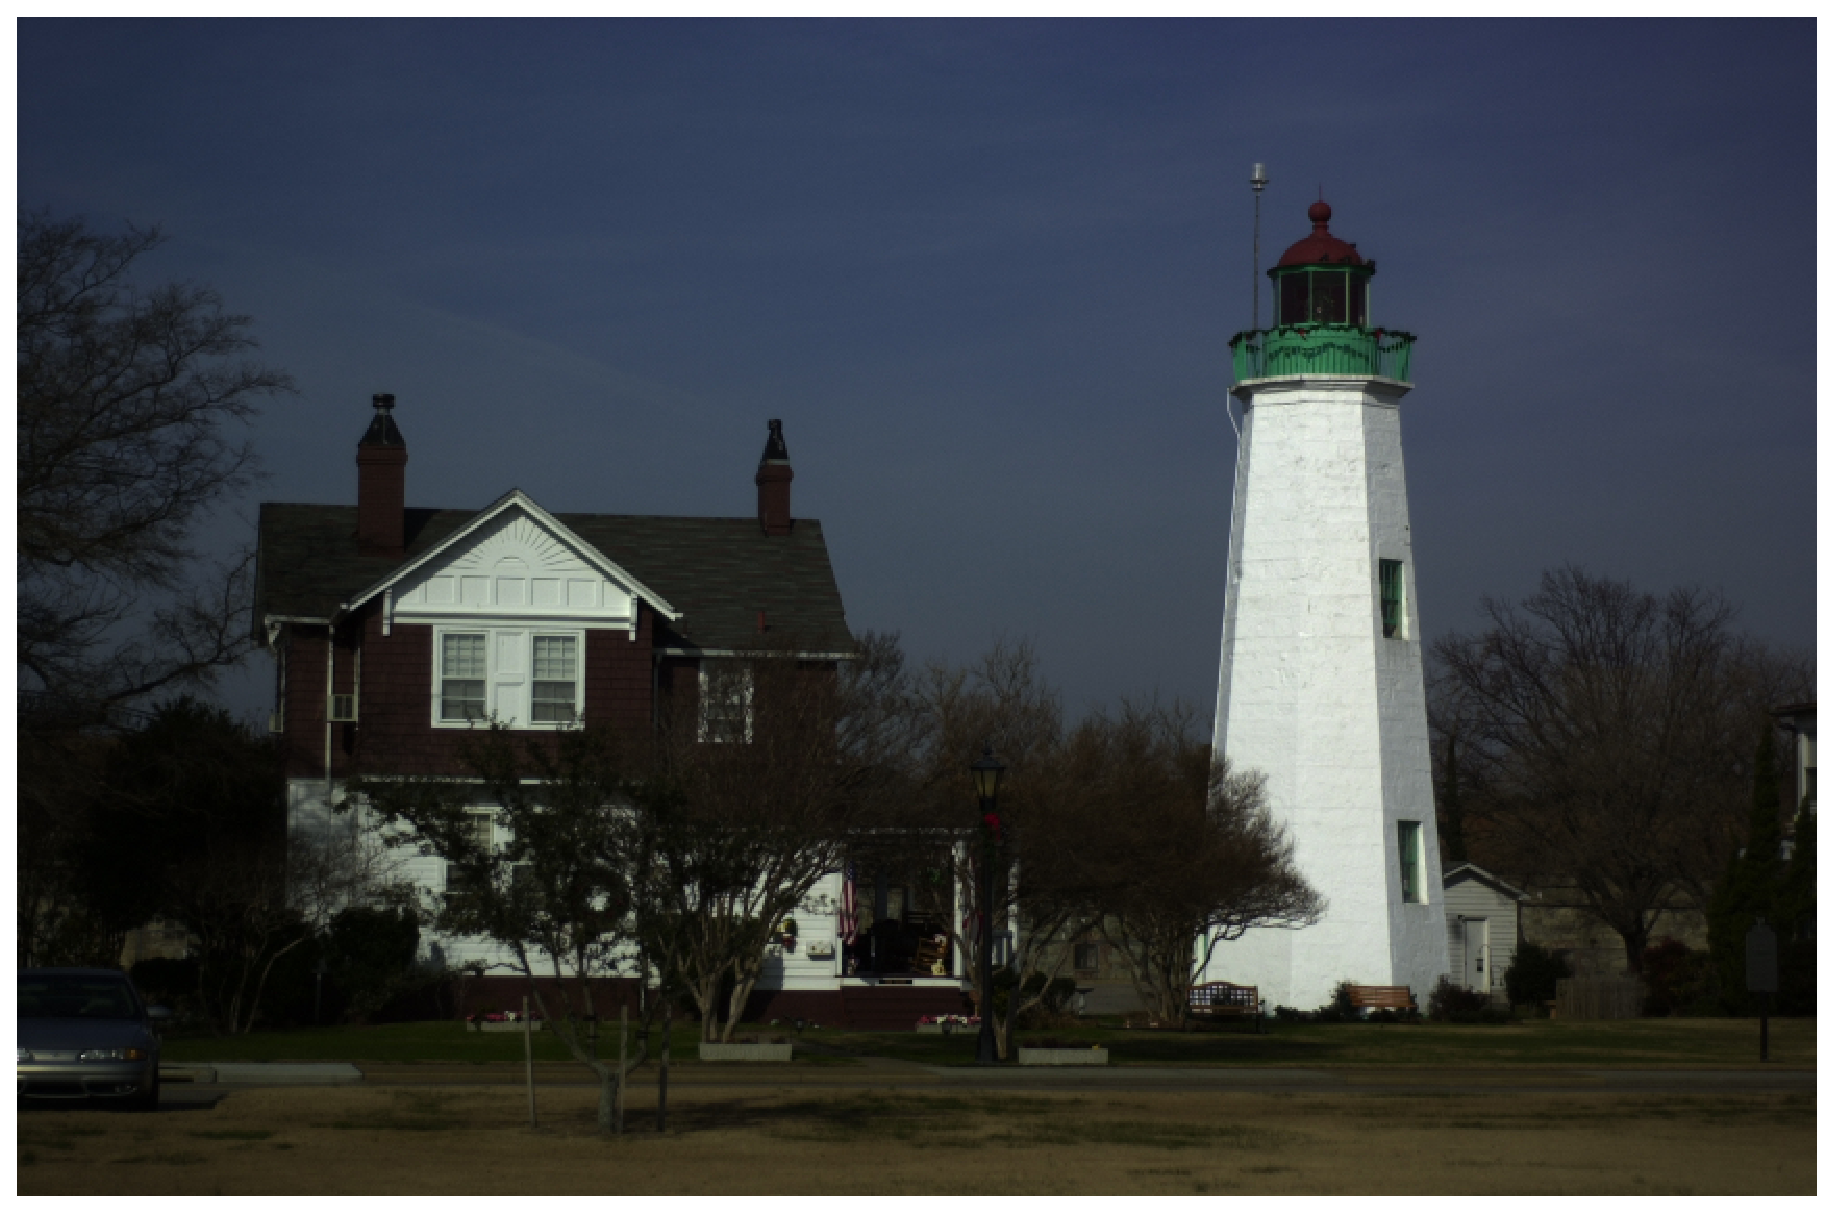
\includegraphics[width=62.5mm]{images/jiep/input.eps}
		\subcaption{Observed image $S$} \label{fig:jiep/input}
	\end{minipage}
	\begin{minipage}[b]{0.5\hsize}
		\centering
		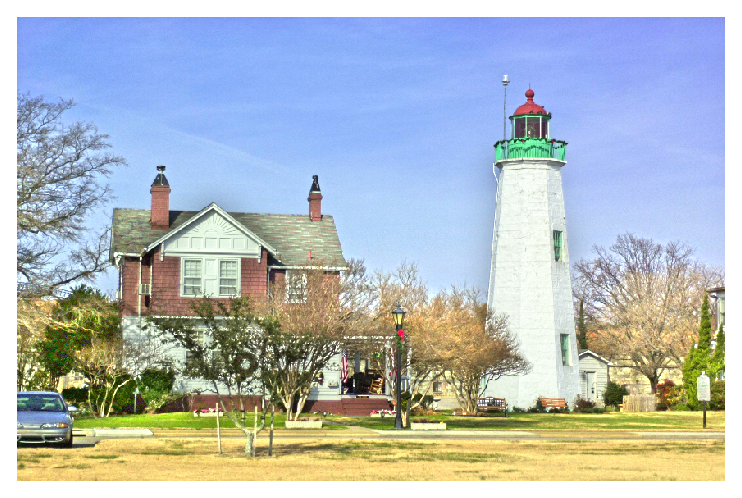
\includegraphics[width=62.5mm]{images/jiep/reflectance.eps}
		\subcaption{Reflectance $R$} \label{fig:jiep/reflectance}
	\end{minipage}
	\begin{minipage}[b]{0.5\hsize}
		\centering
		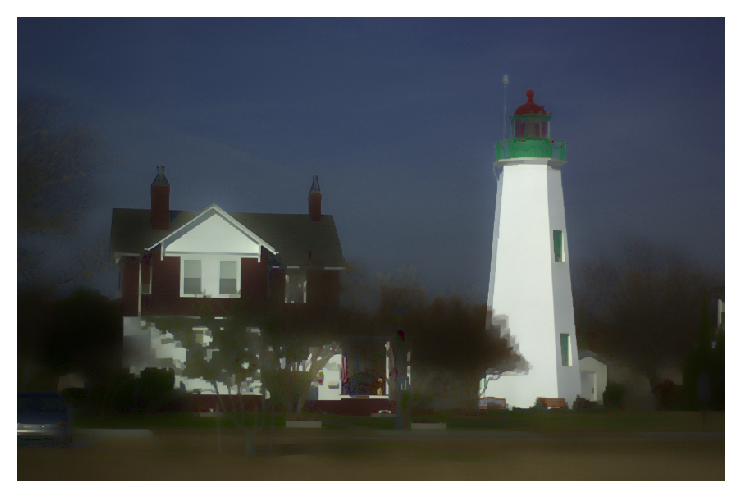
\includegraphics[width=62.5mm]{images/jiep/illumination.eps}
		\subcaption{Illumination $I$} \label{fig:jiep/illumination}
	\end{minipage}
	\begin{minipage}[b]{0.5\hsize}
		\centering
		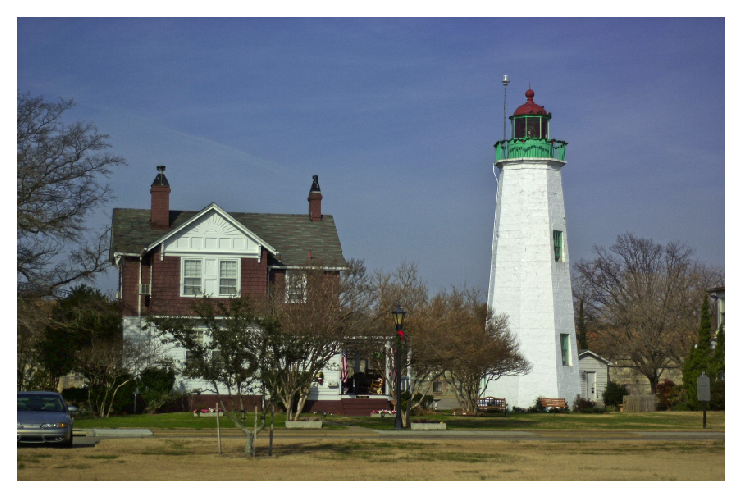
\includegraphics[width=62.5mm]{images/jiep/output.eps}
		\subcaption{Enhanced image $\hat{S}$} \label{fig:jiep/output}
	\end{minipage}
	\caption{The images represent the result of JieP \cite{jiep}.}
	\label{fig:jiep/example}
\end{figure}

\section{Consideration of Problems} \label{sec:problems}
These methods can enhance low-light images by solving each minimization optimization problem.
However, these methods have some problems in the enhanced image or the estimated component.
Therefore, in this section, the discussion centers on such problems with connected images.
\begin{itemize}
\item \textbf{SRIE.}
This method is prone to over-smooth the illumination component without preserving the structure information because of the constraint term $L_{2}$ that the illumination should be spatially smooth. 
As a result, as shown in Fig. \ref{fig:problem/srie/reflectance}, the estimated reflectance generates halo effect along with edge regions that have large intensity gradient. 
Moreover, as can be seen in Fig. \ref{fig:variational/reflectance}, in the estimated reflectance, much noise remain in dark regions and over-enhancement cause in bright regions because the constraint term on the reflectance is lack of the weight to distinguish between dark and bright regions.
\end{itemize}
\begin{itemize}
\item \textbf{JieP.}
This method can significantly take consideration of the constraint term on the illumination, but is not sufficient for the reflectance. Therefore, as can be seen in Fig. \ref{fig:problem/jiep/reflectance}, the estimated reflectance have much noise in dark regions and over-enhance in bright regions. Moreover, the constraint term on the illumination adopts L1 norm regularization, so that it may damage structure information too much in the estimated illumination.
\end{itemize}

%----Problemsの図---- %
\begin{figure}[tb]
	\begin{minipage}[b]{1.0\hsize}
		\centering
		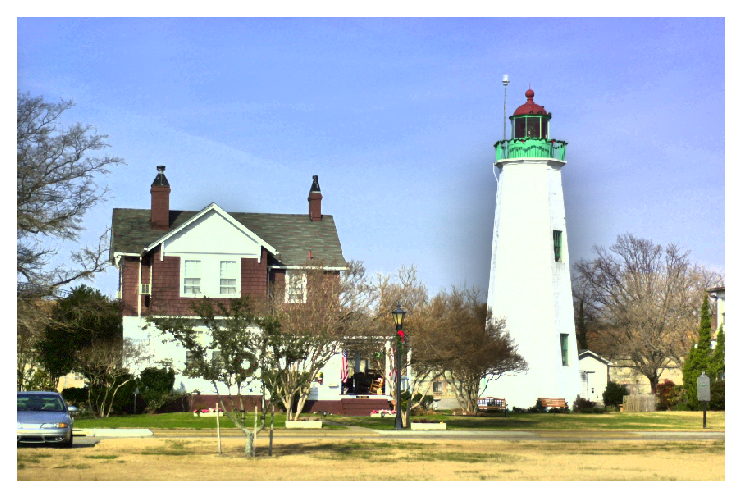
\includegraphics[width=0.65\hsize]{images/problems/srie/reflectance.eps}
		\subcaption{Reflectance (SRIE)} \label{fig:problem/srie/reflectance}
	\end{minipage}\\
	\begin{minipage}[b]{1.0\hsize}
		\centering
		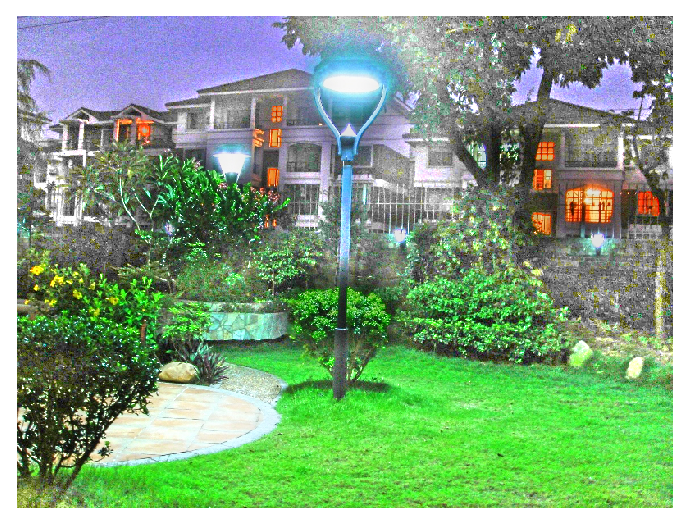
\includegraphics[width=0.65\hsize]{images/problems/jiep/reflectance.eps}
		\subcaption{Reflectance (JieP)} \label{fig:problem/jiep/reflectance}
	\end{minipage}
	\caption{The images represent each problem of these methods.}
	\label{fig:problems}
\end{figure}
\cleardoublepage
%%%%%%%%%%%%%%%%%%%% Proposed Method %%%%%%%%%%%%%%%%%%%%
\chapter{Proposed Method}
\label{sec:proposed}
In this section, the discussion centers on the proposed method which improves the problems described in Sec.\ref{sec:problems}.
First, a mixture $L_{2}$ - $L_{p}$ variational retinex model which further considers the feature of the reflectance and illumination is introduced in Sec. \ref{sec:L2-LP}. 
Next, an adaptive texture map which selectively constrain noise amplification in dark regions and over-enhancement in bright regions is described in Sec. \ref{sec:adaptive}. 
Finally, the solution of the proposed minimization optimization equation is mentioned in Sec. \ref{sec:solution}.\par
Fig. \ref{fig:proposed/flowchart} shows the flowchart of the proposed method.
To explain the flow of the proposed method briefly, the proposed method obtains a low-light image and an initialized illumination which is called the bright channel prior. Next, the proposed method converses a low-light image to HSV-Color scale and extract only value (V) channel. The proposed method iteratively solves sub-problems related with the reflectance and illumination and gets their component which meet the constraints are appropriate for each component. Finally, the proposed method multiply the estimated reflectance and illumination, converses the obtained enhanced image to RGB-Color space.

%----提案手法のフローチャート---- %
\begin{figure}[tb]
	\centering
	\includegraphics[width=1.0\hsize]{images/proposed/flowchart.eps}
	\caption{The image represents the flowchart of the proposed method. (i)The proposed method changes the constraint terms further considered the characteristics for each component. (ii)The proposed method generates adaptive texture map to constrain noise  amplification and over-enhancement in the estimated reflectance. } \label{fig:proposed/flowchart}
\end{figure}

\section{Mixture L2-LP Variational Model} \label{sec:L2-LP}
The conventional methods adopt a $L_{1}$ norm to the constraint term on the reflectance, but the fine detail of the estimated reflectance are susceptible to be damaged. Furthermore, by adopting a $L_{2}$ norm to the constraint term on the illumination, the estimated illumination over-smooths and loss the structure information. Therefore, the proposed method adopts $L_{2}$ - $L_{P}$ norm regularization to each constraint term in order to estimate the reflectance as much as possible to preserve fine detail and estimate the illumination as much as possible to keep the structure information while removing texture component.
The new joint optimization equation is given as:
\begin{equation}
E(I, R) = \argmin_{R, I} \|R \circ I - S\|_{2}^{2} + \alpha \left \|\frac{\nabla{I}}{\frac{1}{\Omega}\Sigma_{\Omega}\nabla{I}+\epsilon}\right\|_{p}^{p} + \beta \|W \circ \nabla{R}\|_{2}^{2} + \gamma \|I - B\|_{2}^{2}, \label{eq:proposed/equation}
\end{equation}
where $\| \cdot \|_{p}$ denotes the $L_{p}$ norm regularization term $(0 < p \leq 2)$, and $W$ is the adaptive texture map related to the reflectance $R$.\par
As described in \cite{l2-lp}, a block coordinate descent \cite{block} is used in order to find an optimal solution to the non-convex objective function $(\ref{eq:proposed/equation})$. Since the $L_{p}$ regularization term causes non-smooth optimization, the proposed method adopts an iteratively re-weighted least square (IRLS) method \cite{iterate} and rewrite the second term in $(\ref{eq:proposed/equation})$ as:
\begin{equation}
\left \|\frac{\nabla{I}}{\frac{1}{\Omega}\Sigma_{\Omega}\nabla{I}+\epsilon}\right\|^{p} = \|U \circ \nabla{I}\|^{2}, \label{eq:approximation}
\end{equation}

\begin{align}
U &= \left \{
	\begin{array}{ll}
	\frac{1}{\xi^{2-p}}, 
	& \left |\frac{\nabla{I}}{\frac{1}{|\Omega|} \sum_{\Omega} \nabla{I} } \right| < \xi\\
	\frac{\left |\Sigma_{\Omega} \nabla{I} \right|^{2-p}}{\left |\nabla{I} \right|^{2-p}} \frac{1}{\left |\Sigma_{\Omega} \nabla{I} \right|^{2}},
	& \rm{otherwise}
	\end{array}
\right.\\
  &= \left \{
  	\begin{array}{ll}
  	\frac{1}{\xi^{2-p}}, 
  	& \left |\frac{\nabla{I}}{\frac{1}{|\Omega|} \sum_{\Omega} \nabla{I} } \right| < \xi\\
  	\frac{1}{\left |\Sigma_{\Omega} \nabla{I} \right|^{p} \left |\nabla{I} \right|^{2-p}},
  	& \rm{otherwise}
  	\end{array}
\right. \label{eq:lp_shape}
\end{align}
where the variable $u$ is only approximate variable. This is because the Eq. \ref{eq:approximation} uses a $L_{2}$ norm format $\Phi(\frac{\nabla{I}}{\frac{1}{\Omega}\Sigma_{\Omega}\nabla{I}+\epsilon};\xi)$ based on \cite{l0-sparse} to approximate the $L_{0} $ norm function. As can be seen in Fig. \ref{fig:nom_p/comparison}, the red curve can approximate the most sparse $L_{0}$ function. Therefore, the proposed method can remove fine textures detail and preserve meaningful salient structures in the estimated illumination. As shown in Fig. \ref{fig:nom_p/graph_norm_p}, with the decease of the value $\xi$, the $L_{p}$ norm function is getting close to the $L_{0}$ function. Therefore, large-$\xi$ are more convex-like and easy to optimize, in contrast, small-$\xi$ are more steep and difficult to optimize.\par
Fig. \ref{fig:comparison_p} shows the effect of changing the value of $p$ in the range ($0 < p \leq 2$) in the estimated illumination. As the value of $p$ decreases, the estimated illumination leaves smooth and texture-less. Concomitantly, the estimated reflectance contains more rich textures detail. In particular, when $p=0$, some salient structure information in the estimated illumination may be lost too much, because the $L_{0}$ norm has strong sparsity. 
%----Lpノルムの概形----
\begin{figure}[tb]
\vspace{-15pt}
	\begin{minipage}[b]{0.5\hsize}
		\centering
		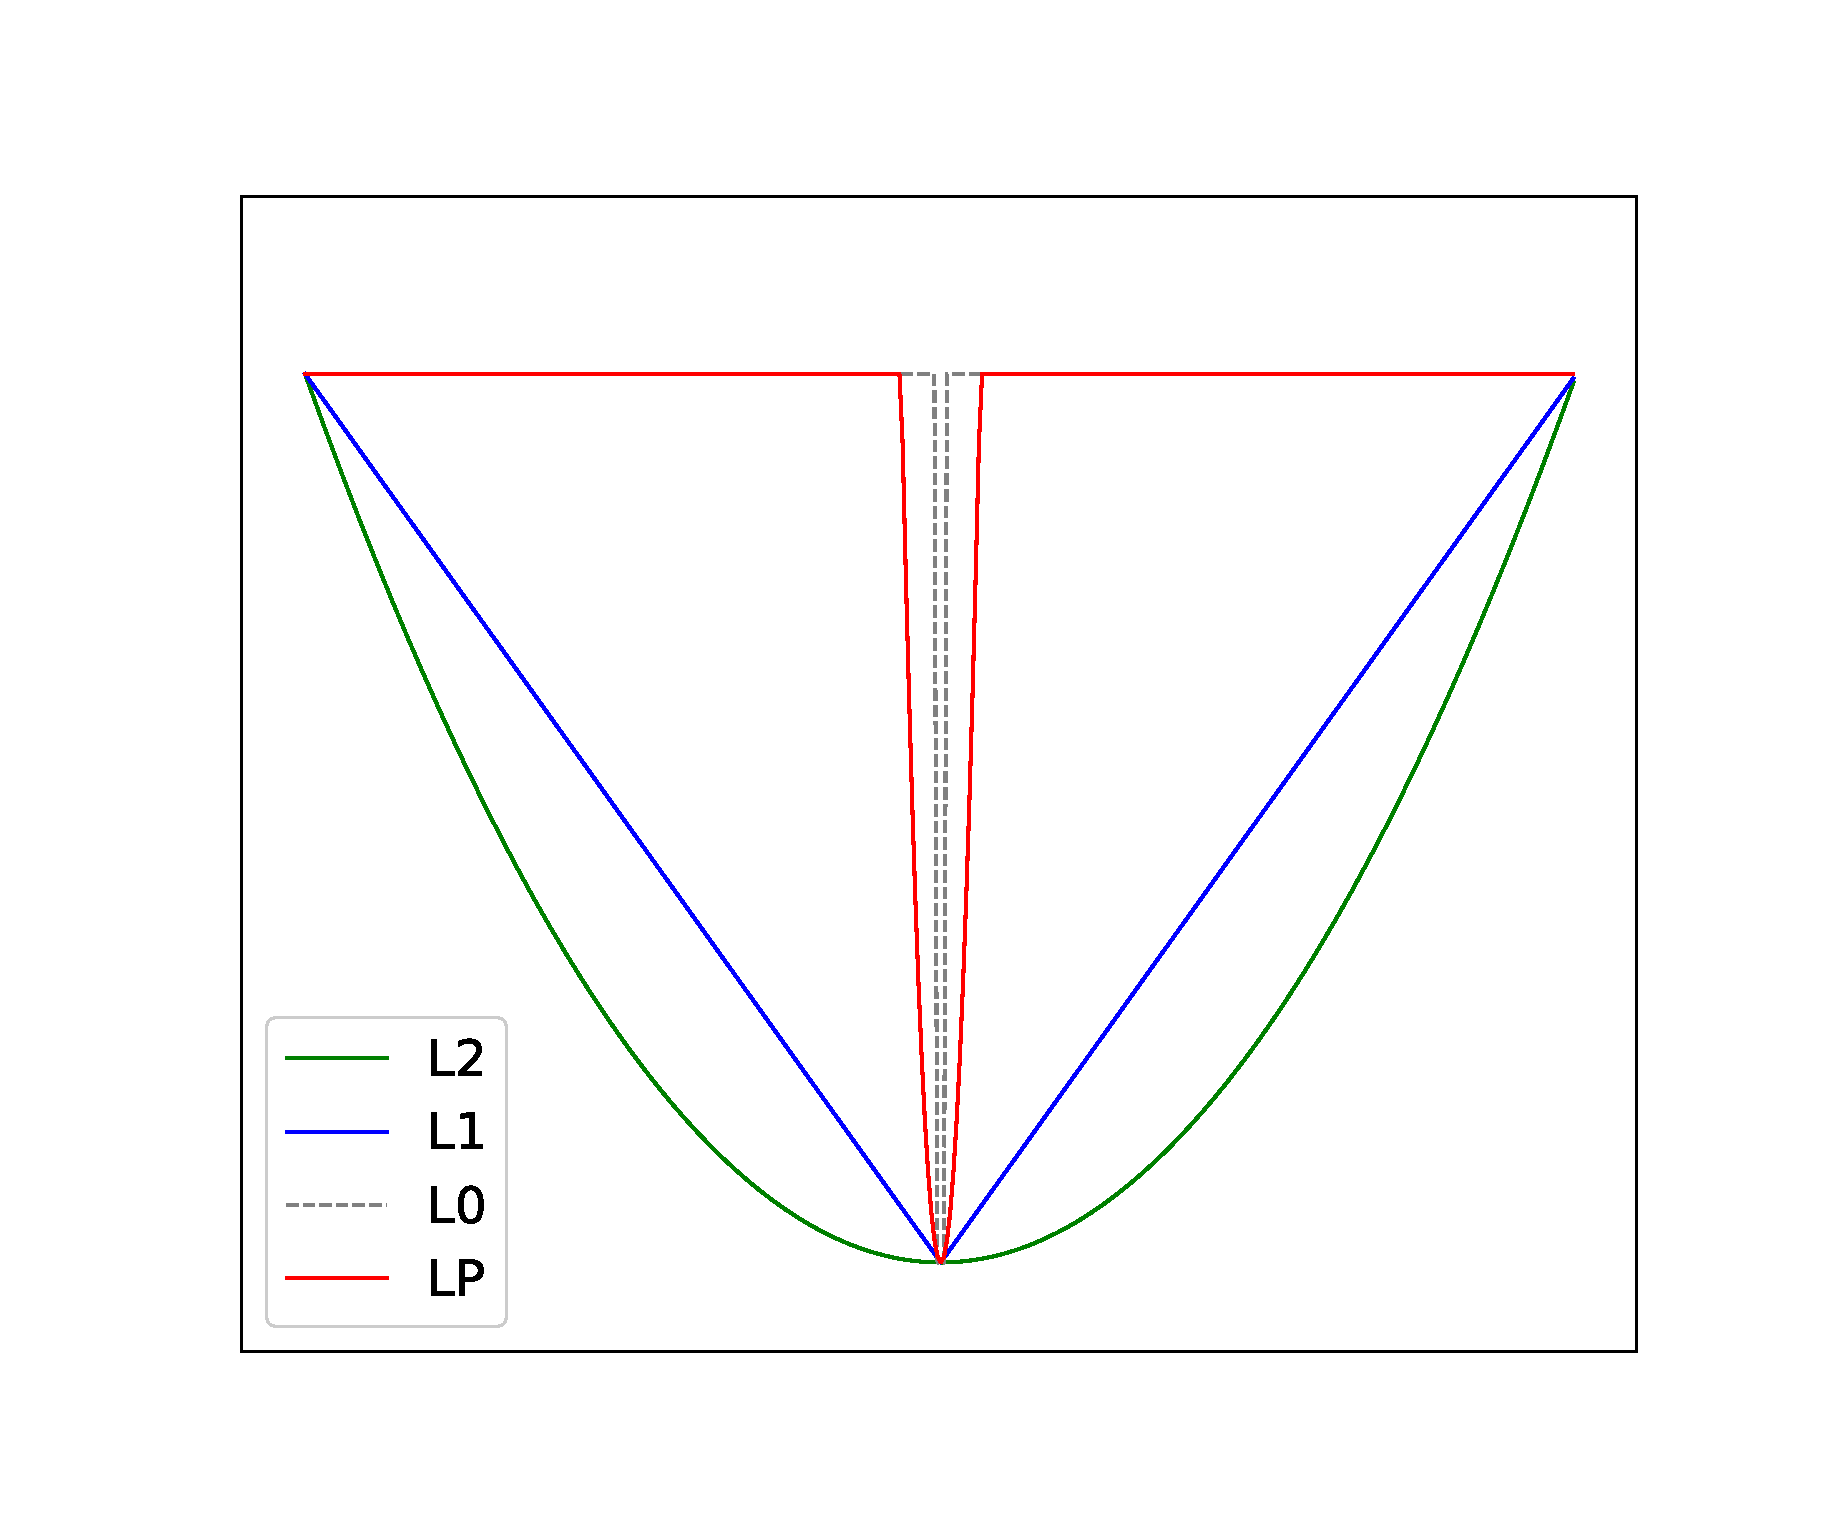
\includegraphics[width=72mm, height = 54mm]{images/norm_p/graph/graph_norm.eps}
		\subcaption{Plots of different penalty functions} \label{fig:nom_p/comparison}
	\end{minipage}
	\begin{minipage}[b]{0.5\hsize}
		\centering
		\includegraphics[width=72mm, height = 54mm]{images/norm_p/graph/graph_norm_p.eps}
		\subcaption{Plots of $L_{p}$ norm for different values $p$} \label{fig:nom_p/graph_norm_p}
	\end{minipage}
	\caption{The images represent various plots about the $L_{p}$ norm, when $p \approx 0$.}
	\label{fig:graph_lp}
\end{figure}
%----ノルムpによる推定比較---- %
\begin{figure*}[tb]
\centering
	\begin{minipage}[b]{0.32\hsize}
	\centering
	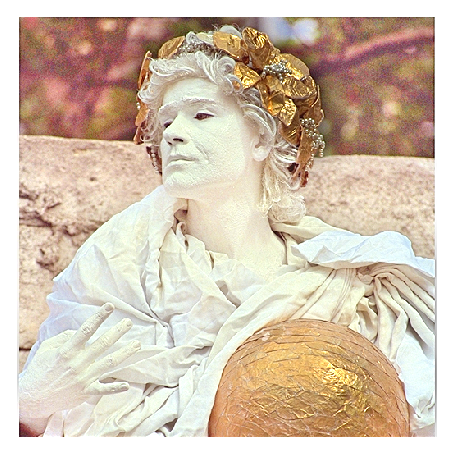
\includegraphics[width=49mm, height = 49mm]{images/norm_p/reflectance/p06.eps}
	\end{minipage}
	\begin{minipage}[b]{0.32\hsize}
	\centering
	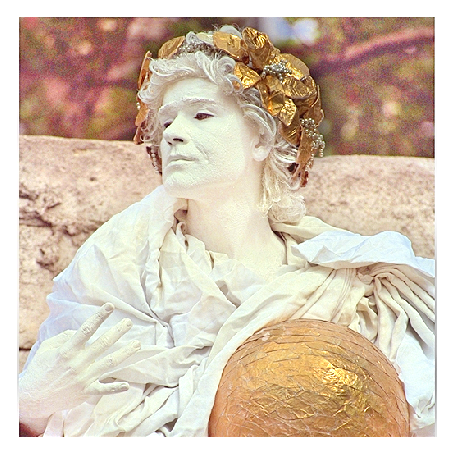
\includegraphics[width=49mm, height = 49mm]{images/norm_p/reflectance/p10.eps}
	\end{minipage}
	\begin{minipage}[b]{0.32\hsize}
	\centering
	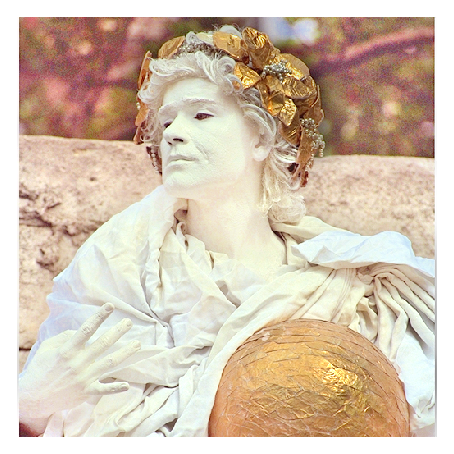
\includegraphics[width=49mm, height = 49mm]{images/norm_p/reflectance/p20.eps}
	\end{minipage}\\
	\vspace{1.5mm}
	\begin{minipage}[b]{0.32\hsize}
	\centering
	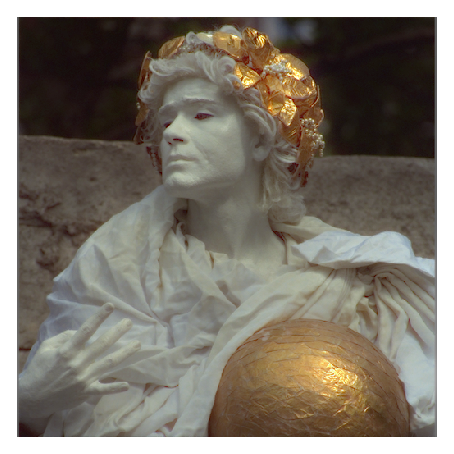
\includegraphics[width=49mm, height = 49mm]{images/norm_p/illumination/p06.eps}
	\subcaption{$p$=0.6} \label{fig. p-04}
	\end{minipage}
	\begin{minipage}[b]{0.32\hsize}
	\centering
	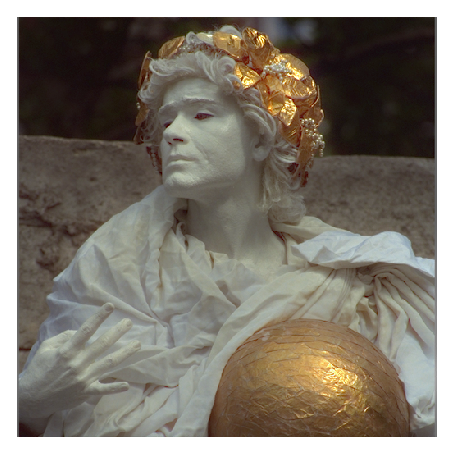
\includegraphics[width=49mm, height = 49mm]{images/norm_p/illumination/p10.eps}
	\subcaption{$p$=1.0} \label{fig. p-10}
	\end{minipage}
	\begin{minipage}[b]{0.32\hsize}
	\centering
	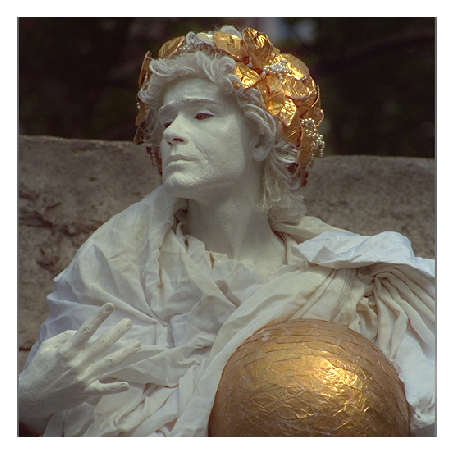
\includegraphics[width=49mm, height = 49mm]{images/norm_p/illumination/p20.eps}
	\subcaption{$p$=2.0} \label{fig. p-20}
	\end{minipage}
	\caption{Comparison of decomposition results for different values of norm $p$. ((a)-(c) top: reflectance, bottom: illumination)}
	\label{fig:comparison_p}
\end{figure*}

\section{Adaptive Texture Map} \label{sec:adaptive}
The discussion centers on the effect of the adaptive texture map using as the weight of the constraint term on the reflectance. Discussed in Sec. \ref{sec:retinex}, reflectance component contains rich details. However, when a low-light image is enhanced, noise hidden in dark regions amplifies and over-enhancement cause in bright regions in the estimated reflectance. Therefore, the weight which controls noise amplification and over-enhancement is necessary for the constraint term on the reflectance. In addition, the preferable reflectance's gradients should be smooth in homogeneous regions while undamaged at edges and texture regions. Thus, when estimating the reflectance, the weight which can recognize more texture regions is required. Fig. \ref{fig:adaptive/classification} shows the summary of the above discussion.
Then, the adaptive texture map $W$ is set so that the third term performs strong noise reduction in dark and homogeneous regions, while it performs weak noise reduction in bright and textures regions. 
The formulation of $W$ is given as:
\begin{equation}
W_{d} = W_{B} \circ A_{d}, \label{eq: adaptive_texture}
\end{equation}
where $d$ represents horizontal ($h$) and vertical ($v$) directions, and $W_{B}$ represents an initial estimated weight map by inverting the normalized bright channel, and $A_{d}$ represents a texture map that effectively distinguish between homogeneous and textures regions.\par
In the same way as in \cite{activation}, given an observed low-light image, $W_{B}$ can selectively assign different values according to BCP since the estimated bright channel contains large values in bright regions and vice versa. 
Thus, $W_{B}$ is given as:
\begin{equation}
W_{B} = 1.0 - \max_{c \in \{r, g, b\}}S^{c}. \label{eq: initial_weight}
\end{equation}
Fig. \ref{fig:adaptive/wb} shows the image of $W_{B}$. Since smaller weight values are assigned in bright regions, $W_{B}$ performs the weaker noise reduction. In contrast, stronger noise reduction is performed in dark regions.\par
 
Moreover, the texture map $A_{d}$ is set as the inverse of the $a_{r}$-th power of the absolute value of a mean local variation (MLV) \cite{jiep}, so that it can significantly distinguish between homogeneous regions and textures regions:
\begin{equation}
A_{d} = \frac{1}{\left |\frac{1}{|\Omega|}\sum_{\Omega}\nabla_{d}{R} \right|^{a_{r}} + \epsilon}, \label{eq: mlv}
\end{equation}
where $a_{r} (< 1)$ is an exponential parameter to adjust the awareness of textures for the reflectance.
As shown in Fig. \ref{fig:mlv_change}, when $a_{r}=1.0$, the texture map $A_{d}$ extracts salient edges but little texture component. In contrast, when $a_{r}=0.5$, it extract both salient edges and rich texture component. Therefore, using the texture map, $W$ performs weaker noise reduction in both edges and texture regions, on the other hand, stronger noise reduction in homogeneous regions.\par
Here, the discussion centers on the effectiveness of the adaptive texture map using Fig. \ref{fig:adaptive/effectiveness}.
As shown in the yellow and green square, the estimated reflectance with $W$ can suppress noise amplification in dark regions and over-enhancement in bright regions more than without $W$. This is because $W_{B}$ can significantly assign different values between dark and bright regions. 
Next, in order to confirm the effectiveness of the texture map $A_{d}$, the edge magnitude in the red square is calculated:
\begin{equation}
M(h, v) = \sqrt{G_{h} ^{2}+ G_{v}^{2}}, \label{eq:maginitude}
\end{equation}
where $G_{h}$, $G_{v}$ represent the horizontal-vertical gradient image respectively. Fig.\ref{fig:adaptive/edge_magnitude} shows the plots of average v-axis edge magnitude. It can be seen the average gradient magnitude with $W$ has larger values and the values fluctuate more rapidly than without $W$. Therefore, the texture map $A_{d}$ contributes to the awareness of textures in the estimated reflectance.
% ----Classificationの図----%
\begin{figure}[tb]
	\centering
	\includegraphics[width=1.0\hsize]{images/adaptive/classification.eps}
	\caption{The image represents the classification of regions where the adaptive texture map has an impact on.} \label{fig:adaptive/classification}
\end{figure}
% ----Weight of BCPの図----%
\begin{figure}[tb]
	\centering
	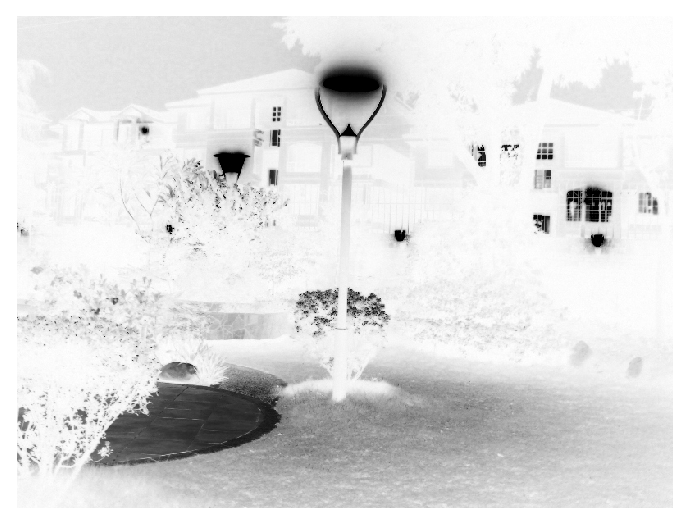
\includegraphics[width=0.5\hsize]{images/adaptive/wb.eps}
	\caption{The image represents $W_{B}$. $W_{B}$ contains smaller values in bright regions, in contrast, larger values in dark regions.} \label{fig:adaptive/wb}
\end{figure}
% ----Texture Mapの図----%
\begin{figure}[tb]
\centering
\begin{minipage}[b]{0.49\hsize}
\centering
\includegraphics[height=0.65\hsize]{images/noise/MLV_10.eps}
\subcaption{MLV ($a_{r}=1.0$)} \label{fig:mlv_normal}
\end{minipage}
\begin{minipage}[b]{0.49\hsize}
\centering
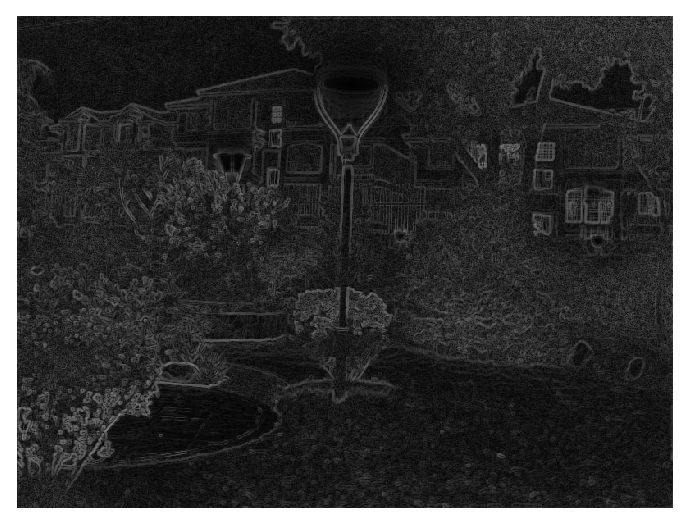
\includegraphics[height=0.65\hsize]{images/noise/MLV_05.eps}
\subcaption{MLV ($a_{r}=0.5$)} \label{fig:mlv_pow}
\end{minipage}
\caption{Comparison of MLV results for different values of $a_{r}$. As the value of $a_{r}$ decreases, MLV can obtain more rich gradient information.}
\label{fig:mlv_change}
\end{figure}
% ----Texture Mapの抑制図----%
\begin{figure}[tb]
\centering
\begin{minipage}[b]{0.49\hsize}
\centering
\includegraphics[width=60mm, height=60mm]{images/adaptive/without.eps}
\subcaption{Reflectance w/o $W$} \label{fig:wo}
\end{minipage}
\begin{minipage}[b]{0.49\hsize}
\centering
\includegraphics[width=60mm, height=60mm]{images/adaptive/with.eps}
\subcaption{Reflectance with $W$} \label{fig:w}
\end{minipage}
\caption{Comparison of reflectance results. (a) the estimated reflectance without $W$; (b) the estimated reflectance with $W$.}
\label{fig:adaptive/effectiveness}
\end{figure}
% ----Edge Magnitudeの図----%
\begin{figure}[tb]
	\centering
	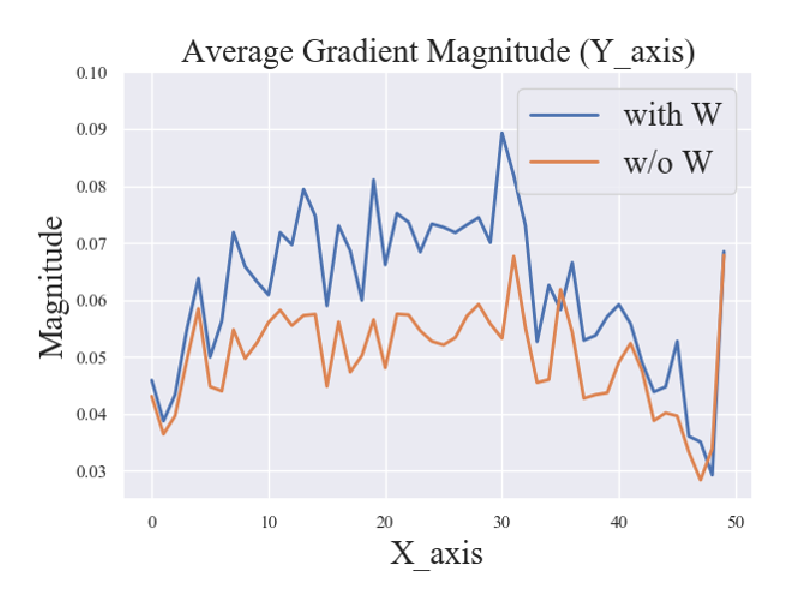
\includegraphics[width=0.5\hsize]{images/adaptive/graph_edge.eps}
	\caption{The image represents the plots of the average edge magnitude.} \label{fig:adaptive/edge_magnitude}
\end{figure}

\section{Solution} \label{sec:solution}
The minimization optimization problem (\ref{eq:proposed/equation}) can be solved by iteratively updating each component. In particular, for the $k$-th iteration of sub-problems.
\begin{enumerate}
\renewcommand{\labelenumi}{\arabic{enumi}).}
\item \textbf{$\boldmath{I}$ sub-problem:} Collecting the terms related to $I$ leads to the following equation (\ref{eq:proposed/equation}):
\begin{equation}
I_{k} = \argmin_{I}\|R_{k-1} \circ I - S\|_{2}^{2} + \alpha\|U \circ \nabla{I}\|_{2}^{2} 
+\lambda \|I - B\|_{2}^{2}. \label{eq: i_subproblem}
\end{equation}
The equation (\ref{eq: i_subproblem}) is transferred to a classic least square problem:
\begin{equation}
i_{k} = \argmin_{i} \|r_{k-1} i - s\|_{2}^{2} + \alpha\|uDi\|_{2}^{2} + \lambda \|i - b\|_{2}^{2}, \label{eq:classic_i_subproblem}
\end{equation}
where $i$ is the vectorized format of $I$ and $D$ contains $D_{h}$ and $D_{v}$, which are the Toeplitz matrices from the discrete gradient operators with forward difference.
The same notation is used for other matrices (r, s, b corresponds to R, S, and B, respectively). By differentiating equation (\ref{eq:classic_i_subproblem}) with respect to $i$, and setting the derivative to $0$, we have the following solution:
\begin{equation}
i_{k+1} = (r_{k-1}r_{k-1}^{T} + \alpha D^{T}uD + \lambda{1})^{-1} (r_{k-1}^{T}s + \lambda{b}). \label{eq: i_solution}
\end{equation}
Then, the obtained $i_{k}$ is reformulated into matrix format $I_{k}$.
\item \textbf{$R$ sub-problem:} After acquiring $I_{k}$ from the above solution, the joint optimization (\ref{eq:proposed/equation}) related to $R$ becomes similar to that of $I$:
\begin{equation}
R_{k} = \argmin_{R}\|R \circ I_{k} - S\|_{2}^{2} + \beta\|W \circ \nabla{R}\|_{2}^{2}. \label{eq: r_subproblem}
\end{equation}
In the same way as in the former derivation, the solution of $R$ is provided as follows:
\begin{equation}
r_{k} = \argmin_{r} \|ri_{k} - s\|_{2}^{2} + \beta\|wDr\|_{2}^{2}, \label{eq:classic_r_subproblem}
\end{equation}
\begin{equation}
r_{k} = (i_{k}i_{k}^{T} + \beta D^{T}wD)^{-1} (i_{k}^{T}s). \label{eq: solution_r_subproblem}
\end{equation}
Similarly, the obtained $r_{k}$ is reformulated into matrix format $R_{k}$.
\end{enumerate}
The values of $I$ and $R$ are updated until $\|I_{k}-I_{k-1}\|/\|I_{k-1}\| \leq \varepsilon$ and $\|R_{k}-R_{k-1}\|/\|R_{k-1}\| \leq \varepsilon$ are simultaneously satisfied. After the estimation of  the reflectance and illumination, a Gamma correction operation is adopted to adjust the illumination. Therefore, the final enhanced image is given as $ S_{enhanced} = R \circ I^{\frac{1}{\gamma^{'}}}, \label{eq_final}$ where the empirical parameter $\gamma^{'}$ is set as 2.2. To preserve color information, the Gamma correction is performed in the HSV domain.

Fig. \ref{fig:proposed/output} shows the result of the proposed method. The proposed method can estimate the illumination as much as possible to smooth and keep the meaningful structure information while removing much textures detail and estimate the reflectance as much as possible to clarify fine textures detail while suppressing noise amplification in dark regions and over-enhancement in bright regions. Therefore, it can be seen the proposed method naturally enhances low-light images.
%----提案手法の結果の図---- %
\begin{figure}[tb]
\centering
	\begin{minipage}[b]{0.49\hsize}
		\centering
		\includegraphics[width=62.5mm]{images/proposed/input.eps}
		\subcaption{Low-Light Image} \label{fig:proposed/input}
	\end{minipage}
	\begin{minipage}[b]{0.49\hsize}
		\centering
		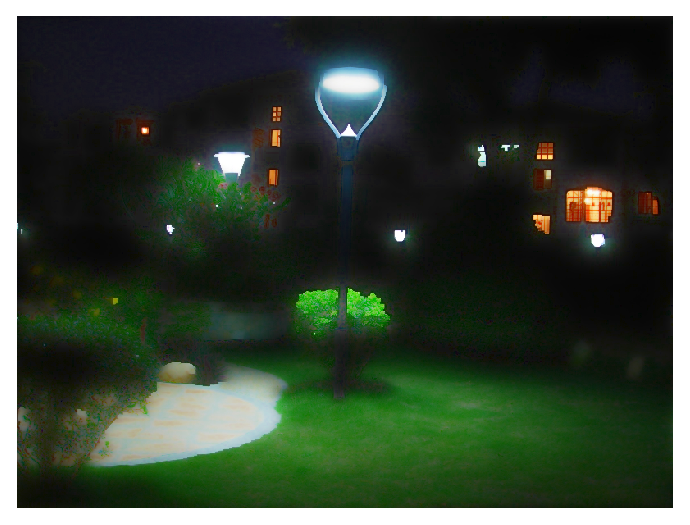
\includegraphics[width=62.5mm]{images/proposed/illumination.eps}
		\subcaption{Illumination} \label{fig:proposed/illumination}
	\end{minipage}
	\begin{minipage}[b]{0.49\hsize}
		\centering
		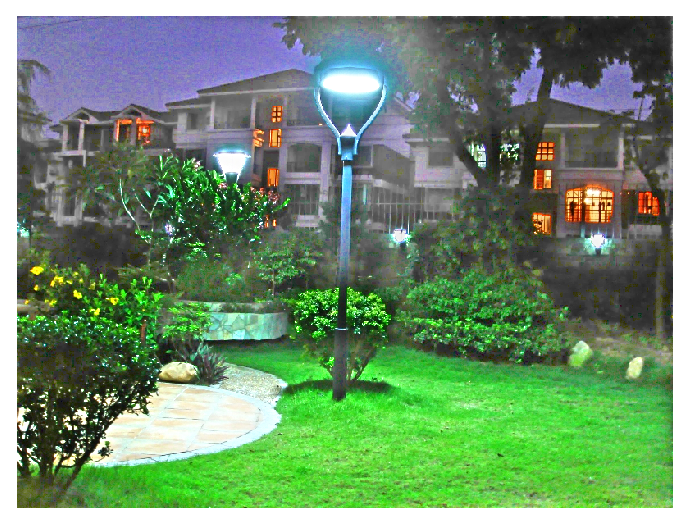
\includegraphics[width=62.5mm]{images/proposed/reflectance.eps}
		\subcaption{Reflectance} \label{fig:proposed/reflectance}
	\end{minipage}
	\begin{minipage}[b]{0.49\hsize}
		\centering
		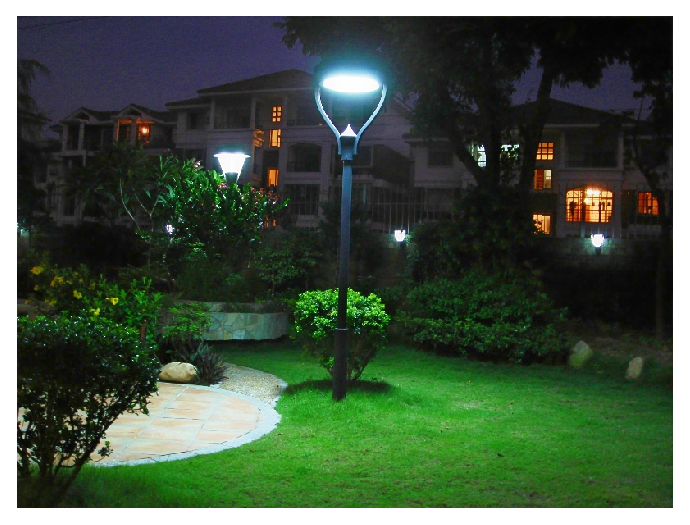
\includegraphics[width=62.5mm]{images/proposed/output.eps}
		\subcaption{Enhanced Image} \label{fig:proposed/enhanced}
	\end{minipage}
	\caption{The images represent the result of the proposed method.}
	\label{fig:proposed/output}
\end{figure}
\cleardoublepage
%%%%%%%%%%%%%%%%%%%% Experiment %%%%%%%%%%%%%%%%%%%%
\chapter{Experiment}
\label{sec:experiment}
This section is devoted to demonstrating the superiority of the proposed method in terms of whether the proposed method can estimate the reflectance and illumination upon considering the characteristics of their component and whether it can naturally enhance low-light images. The word "naturally" means that the methods can suppress over-enhancement and noise amplification when enhancing. 
To this aim, this section is composed of the subsequent five aspects: testing dataset, competing methods, decomposition comparison, qualitative evaluation, and quantitative evaluation.
In this experiment, the empirical parameters as $\alpha=0.007$, $\beta=0.001$, $\lambda=0.25$, $\epsilon=10^{-2}$ are set. In addition, the proposed method is performed on Python implementation on PC with 16GB RAM, Intel Core i7-6700 CPU @ 3.40GHz. 

\section{Comparison of Decomposition} \label{sec:decomposition}
The aim of the section is to evaluate how accurately the proposed method decomposes an observed image into the reflectance and illumination. As described in \cite{retinex}, the illumination should not distort the structure information while keeping smoothness. On the other hand, the reflectance should contain rich detail of an observed image. Although it is necessary to evaluate how much the proposed method estimates their component upon considering their characteristics, the ground truth for their component is difficult to obtain. Therefore, in order to confirm the effectiveness of the proposed method, the proposed method is compared with several state-of-the-art methods: three Retinec-based methods which are implemented in HSV-color space as well as the proposed method, including simultaneous reflectance and illumination estimation (SRIE) \cite{srie}, a weighted variational model (WVM) \cite{wvm}, and a joint intrinsic-extrinsic prior (JieP) \cite{jiep}. The codes of the three methods are downloaded from the author's Github websites and performed with recommended experimental settings.\par
Fig. \ref{fig:decomposition} summarizes the decomposition result of the reflectance and illumination from an observed image. 
SRIE and WVM cannot sufficiently distinguish between reflectance and illumination component, so that the estimated reflectance contains much illumination component. 
Moreover, the estimated illumination breaks the structure of the scene because it is over-smoothed. 
JieP significantly removes the illumination component from the reflectance, but the estimated illumination loses the meaningful structure information too much. 
In summary, he proposed method can sufficiently maintain the structure information with possible texture-less in the estimated illumination. In addition, the proposed method can adaptively reveal textures detail at dark and bright regions in the estimated reflectance.
%----反射と照明の推定比較---- %
\begin{figure*}[htbp]
\centering
	\begin{minipage}[b]{0.49\hsize}
		\centering
		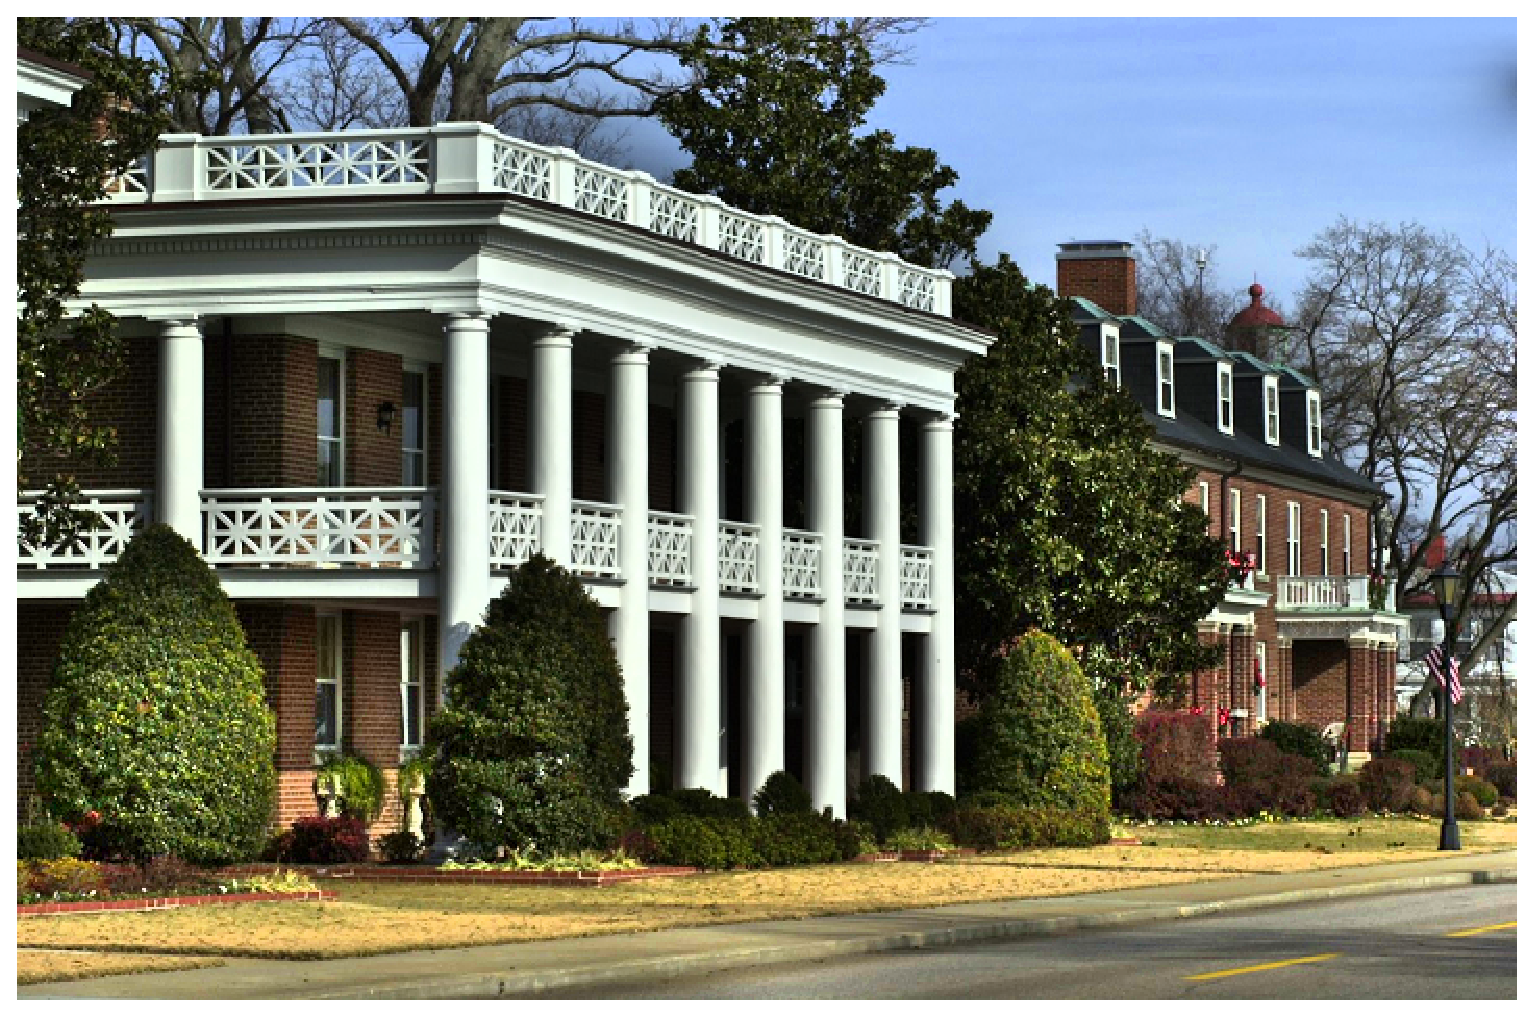
\includegraphics[width=72mm, height=48mm]{images/experiment/decomp/srie/reflectance.eps}
	\end{minipage}
	\begin{minipage}[b]{0.49\hsize}
		\centering
		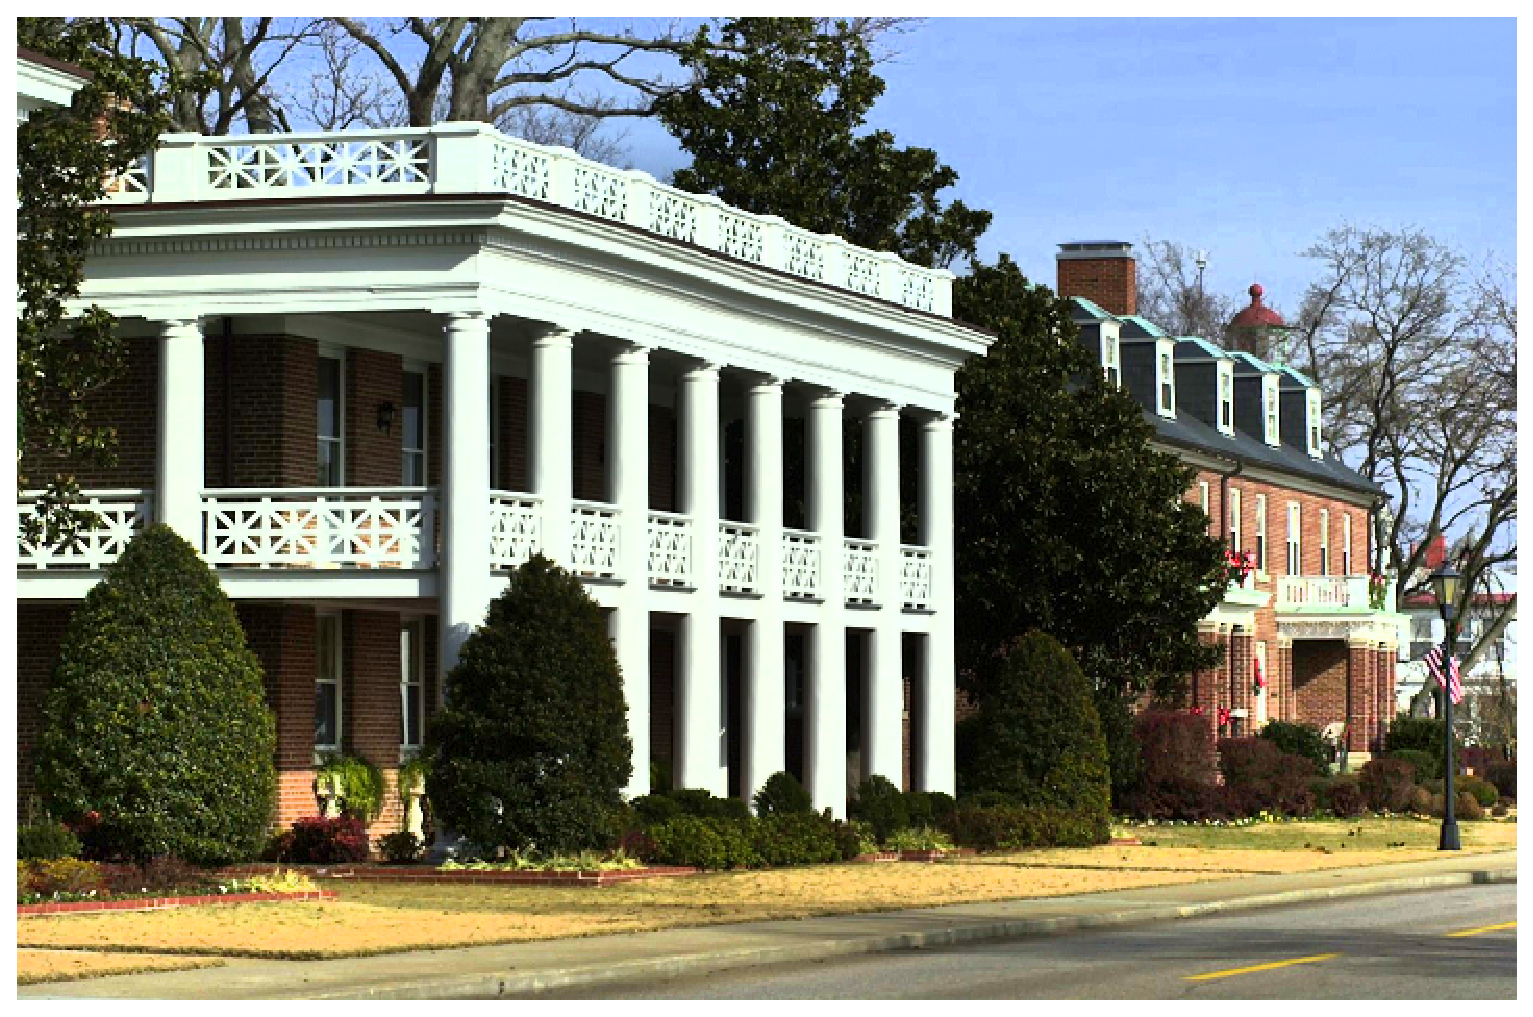
\includegraphics[width=72mm, height=48mm]{images/experiment/decomp/wvm/reflectance.eps}
	\end{minipage} \\
	\vspace{1.5mm}
	\begin{minipage}[b]{0.49\hsize}
		\centering
		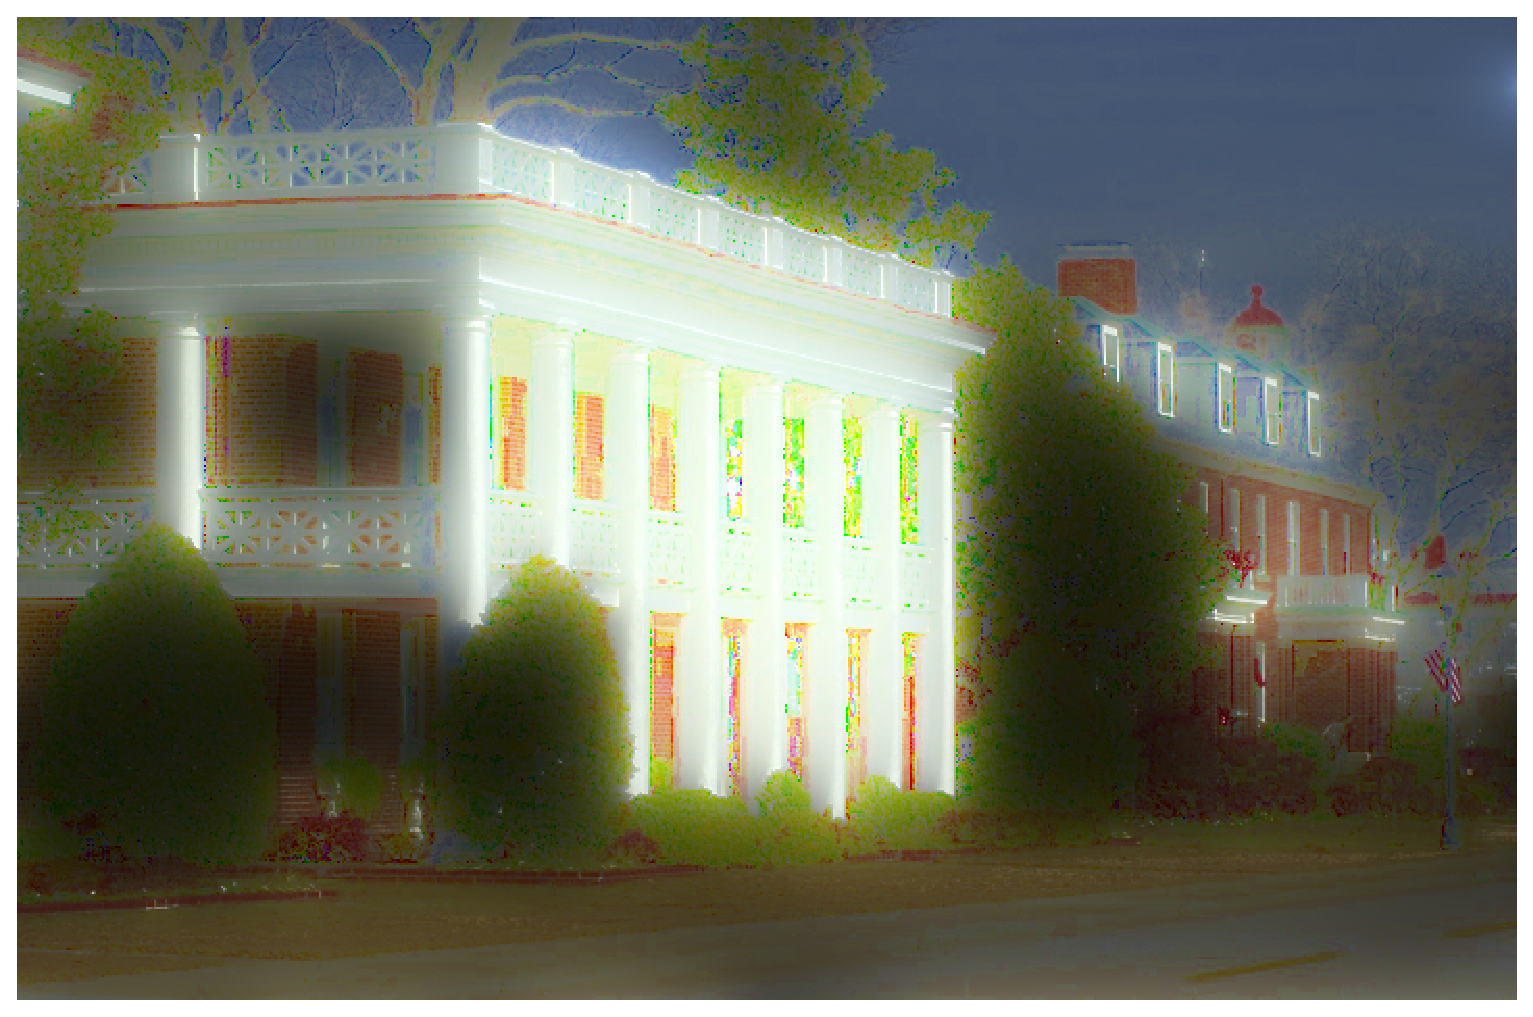
\includegraphics[width=72mm, height=48mm]{images/experiment/decomp/srie/illumination.eps}
		\subcaption{SRIE} \label{fig. decomp_srie}
	\end{minipage}
	\begin{minipage}[b]{0.49\hsize}
		\centering
		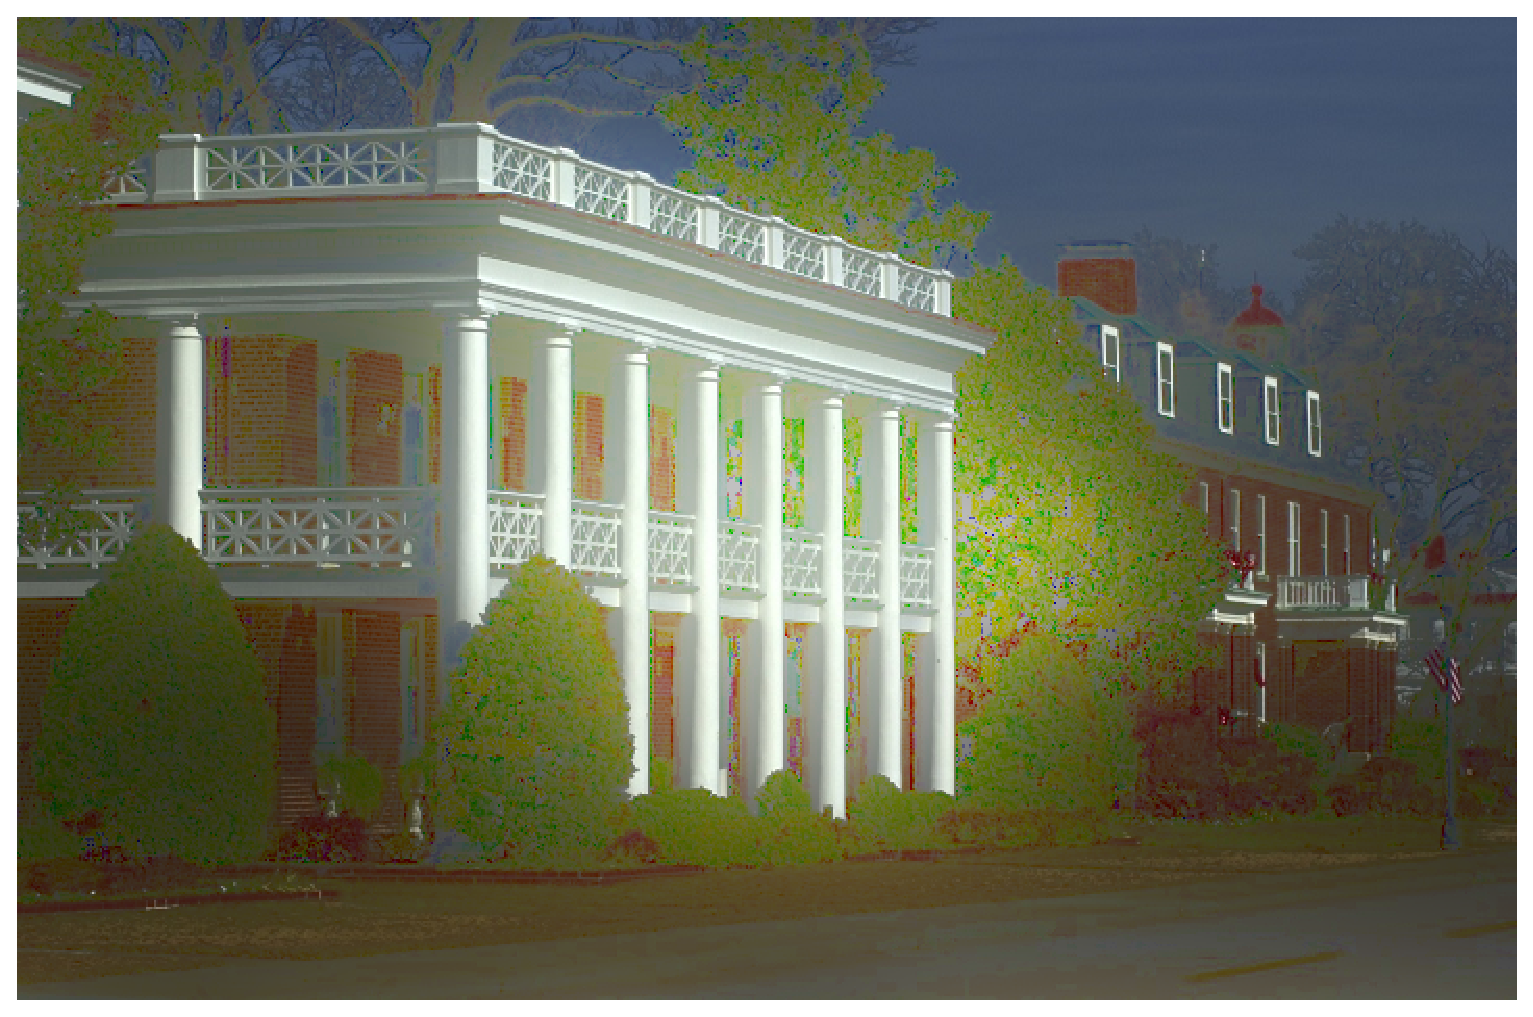
\includegraphics[width=72mm, height=48mm]{images/experiment/decomp/wvm/illumination.eps}
		\subcaption{WVM} \label{fig. decomp_wvm}
	\end{minipage}\\
	\begin{minipage}[b]{0.49\hsize}
	\centering
	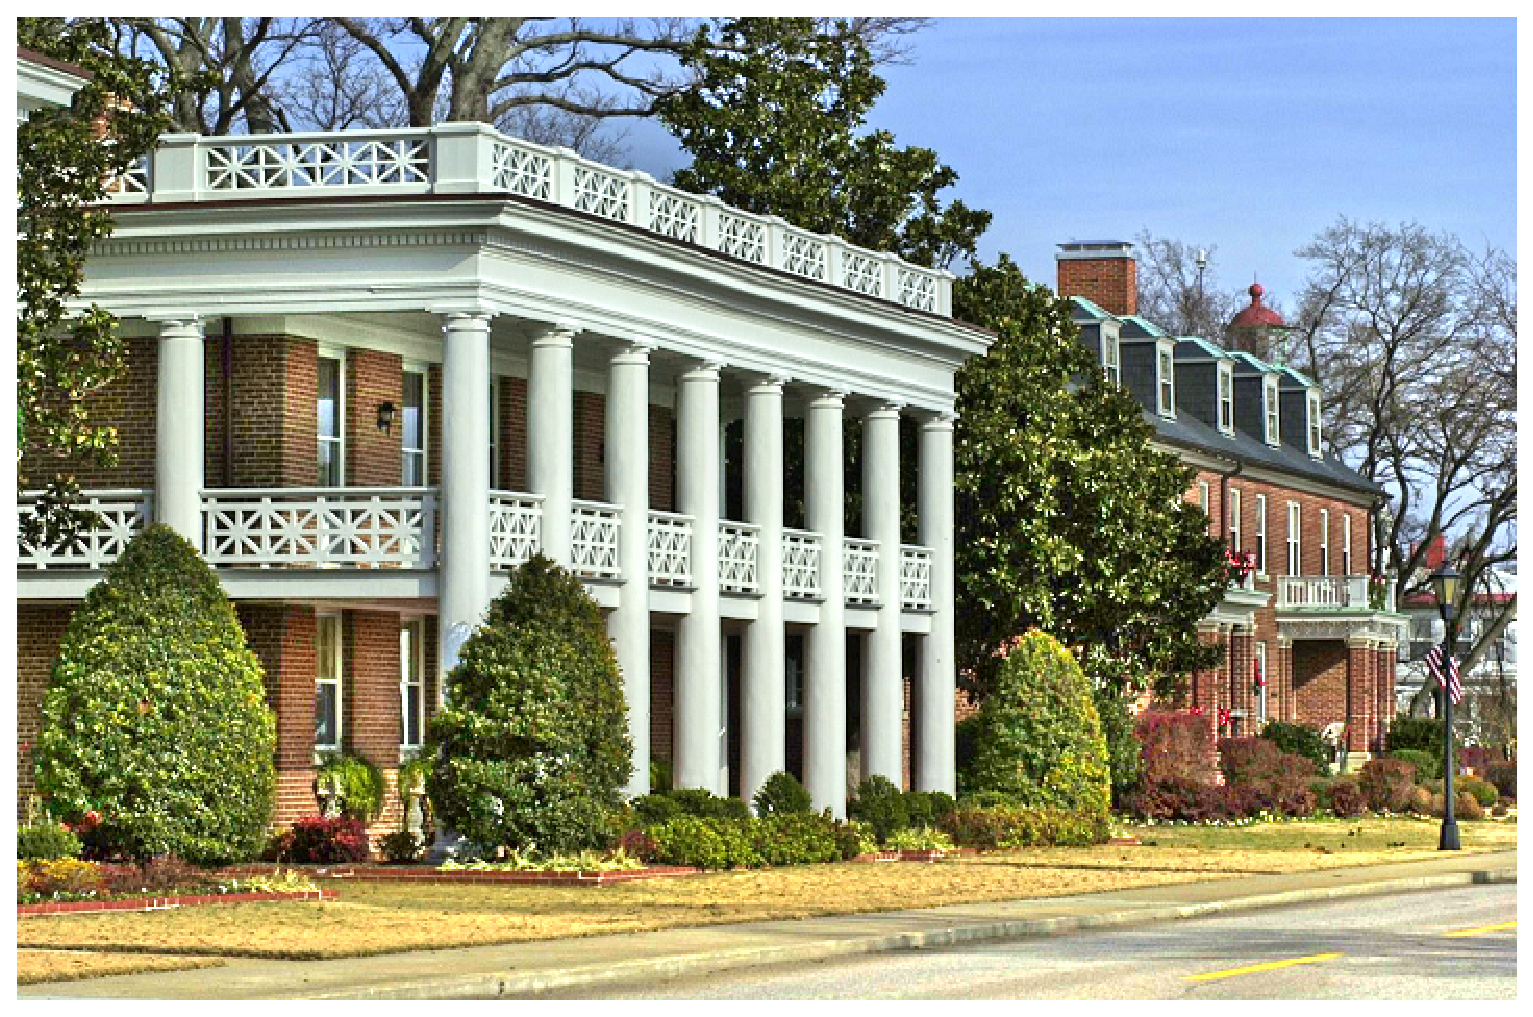
\includegraphics[width=72mm, height=48mm]{images/experiment/decomp/jiep/reflectance.eps}
	\end{minipage}
	\begin{minipage}[b]{0.49\hsize}
	\centering
	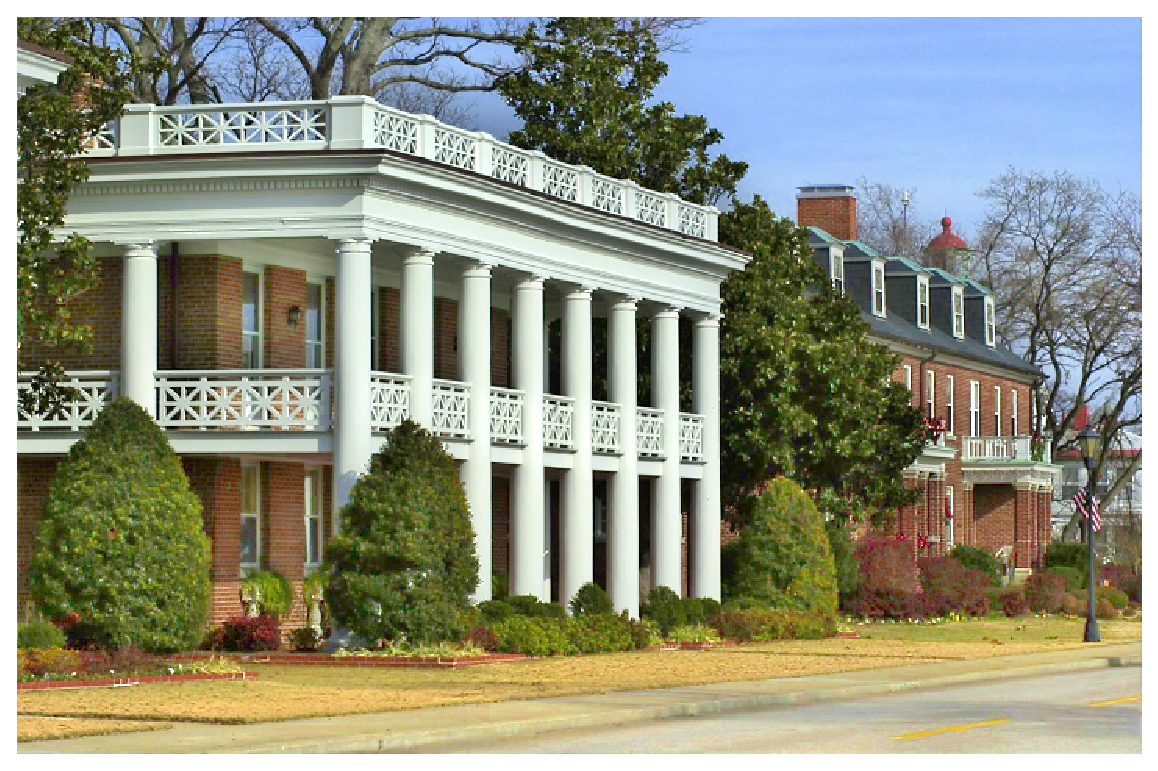
\includegraphics[width=72mm, height=48mm]{images/experiment/decomp/prop/reflectance.eps}
	\end{minipage}\\
	\vspace{1.5mm}
	\begin{minipage}[b]{0.49\hsize}
	\centering
	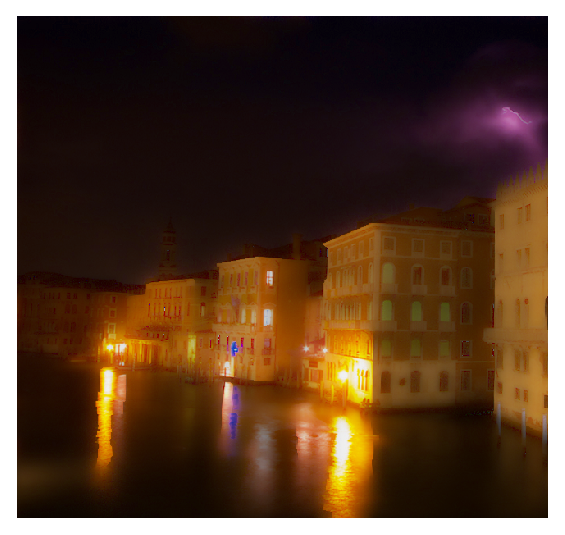
\includegraphics[width=72mm, height=48mm]{images/experiment/decomp/jiep/illumination.eps}
	\subcaption{JieP} \label{fig. decomp_jiep}
	\end{minipage}
	\begin{minipage}[b]{0.49\hsize}
	\centering
	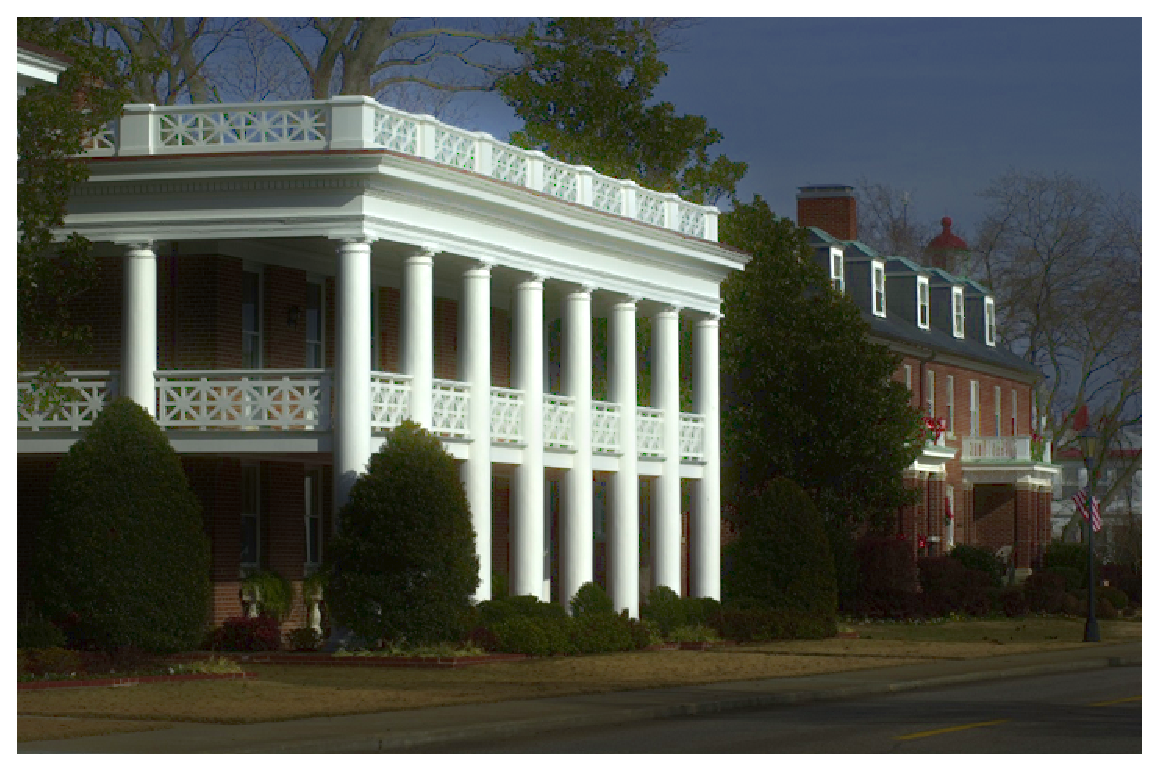
\includegraphics[width=72mm, height=48mm]{images/experiment/decomp/prop/illumination.eps}
	\subcaption{Ours} \label{fig. decomp_prop}
	\end{minipage}
	\caption{Reflectance and illumination decomposed by SRIE, WVM, JieP, and Ours. ((a)-(d) top: reflectance, bottom: illumination)}
	\label{fig:decomposition}
\end{figure*}

\section{Qualitative Evaluation} \label{sec:qualitative}
This section focus on the comparison with the proposed method and several state-of-the-art methods based on the qualitative evaluation. 
%The qualitative evaluation is  to evaluate whether these methods naturally enhance low-light images. The word "naturally" means that the methods can suppress over-enhancement and noise amplification when enhancing. 
Similar to the above comparison of decomposition, several state-of-the-art methods are used: three Retinex methods including SRIE, WVM, and a robust Retinex model (RRM) \cite{rrm}, and non-Retinex method (low-light image enhancement via illumination map estimation (LIME) \cite{lime}). \par
Fig. \ref{fig:qualitative/1} summarizes the low-light image enhancement results of all the competitors for dataset $\#6$. SRIE and WVM generate noticeable halo effects in the edges of the tower. In addition, these methods lose textures detail in bright regions. RRM exhibits an outstanding performance in noise suppression, but the result of the method is likely to be blurry and loses textures detail. LIME shows impressive performance in lighting up dark regions. However, the method often over-enhances the low-light image so that the result loses textures detail too much, specifically in bright regions. In summary, the proposed method can suppress halo effects and over-enhancement. Moreover, the proposed method clarifies more textures detail.\par
Fig. \ref{fig:qualitative/2} summarizes the low-light image enhancement results of all the competitors for dataset $\#7$. SRIE can naturally enhance, but WVM generates severe noise amplification in dark regions. RRM significantly enhances the low-light image while suppressing noise amplification, but the result is so blurry on the entire. LIME illuminates dark regions, but over-enhances in regions with relatively high intensities. In summary, the proposed method achieves good performances in brightness, the awareness of textures detail, and noise suppression.
%----定性評価1の図---- %
\begin{figure*}[htbp]
\centering
	\begin{minipage}[b]{0.49\hsize}
		\centering
		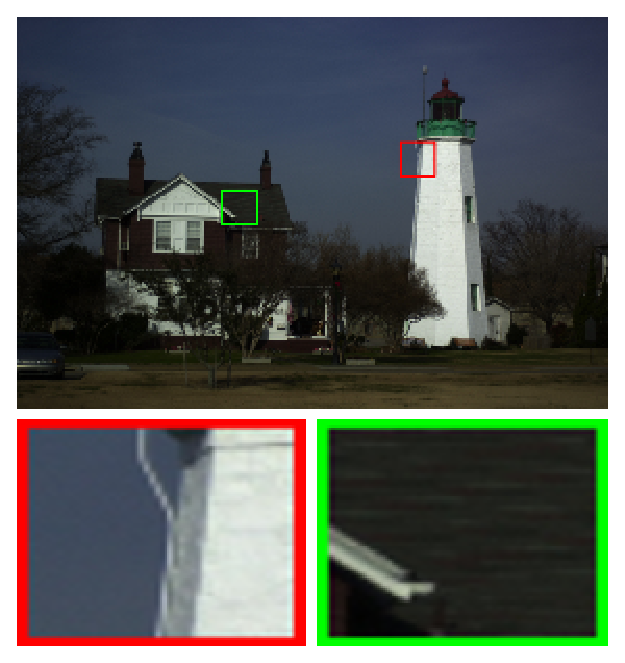
\includegraphics[width=60mm, height=48mm]{images/experiment/qualitative/comp1/input.eps}
		\subcaption{Low-lgiht Image} \label{fig:qualitative/1/input}
	\end{minipage}
	\begin{minipage}[b]{0.49\hsize}
		\centering
		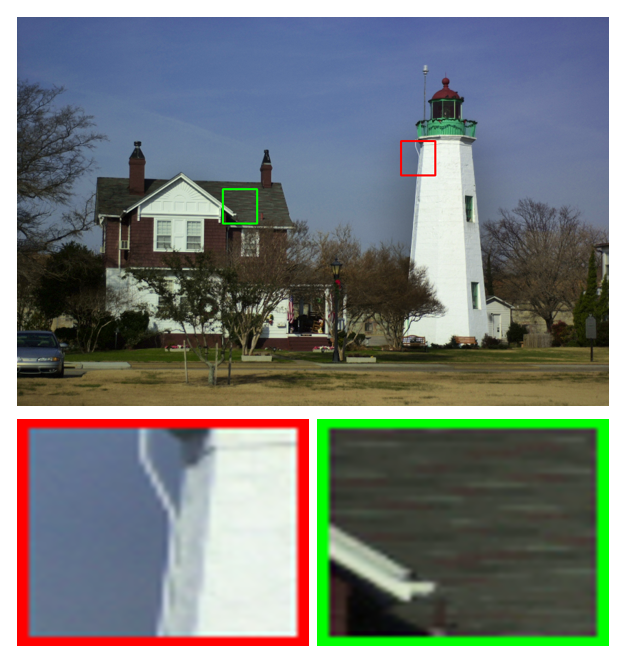
\includegraphics[width=60mm, height=48mm]{images/experiment/qualitative/comp1/srie.eps}
		\subcaption{SRIE} \label{fig:qualitative/1/srie}
	\end{minipage} \\
	\begin{minipage}[b]{0.49\hsize}
		\centering
		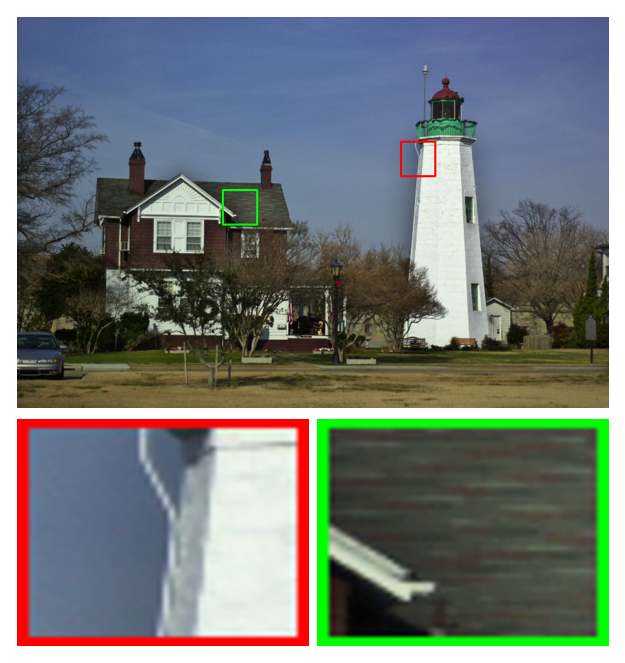
\includegraphics[width=60mm, height=48mm]{images/experiment/qualitative/comp1/wvm.eps}
		\subcaption{WVM} \label{fig:qualitative/1/wvm}
	\end{minipage}
	\begin{minipage}[b]{0.49\hsize}
		\centering
		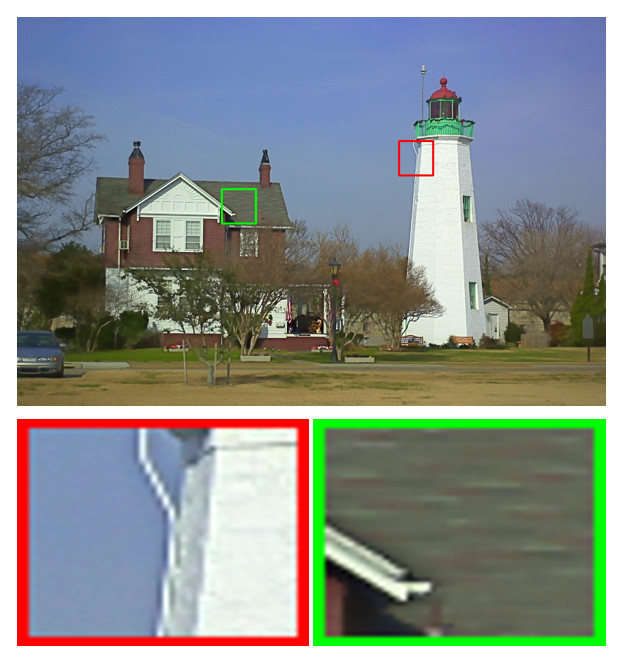
\includegraphics[width=60mm, height=48mm]{images/experiment/qualitative/comp1/rrm.eps}
		\subcaption{RRM} \label{fig:qualitative/1/rrm}
	\end{minipage} \\
	\begin{minipage}[b]{0.49\hsize}
	\centering
	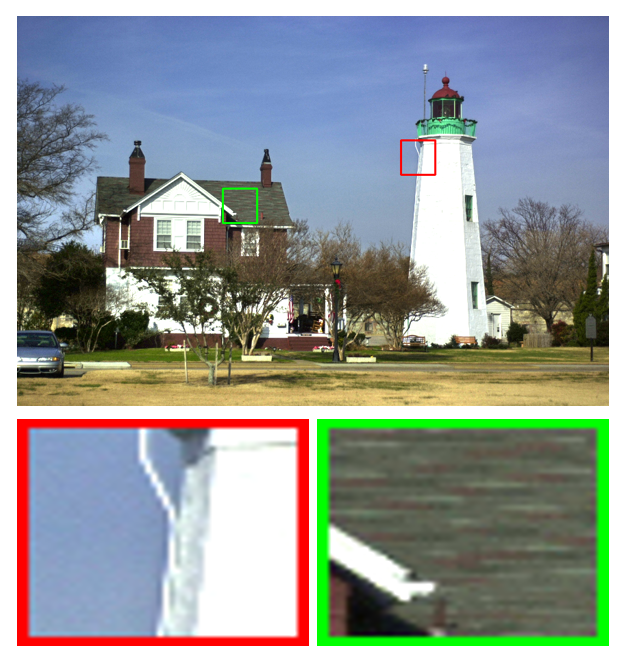
\includegraphics[width=60mm, height=48mm]{images/experiment/qualitative/comp1/lime.eps}
	\subcaption{LIME} \label{fig:qualitative/1/lime}
	\end{minipage}
	\begin{minipage}[b]{0.49\hsize}
	\centering
	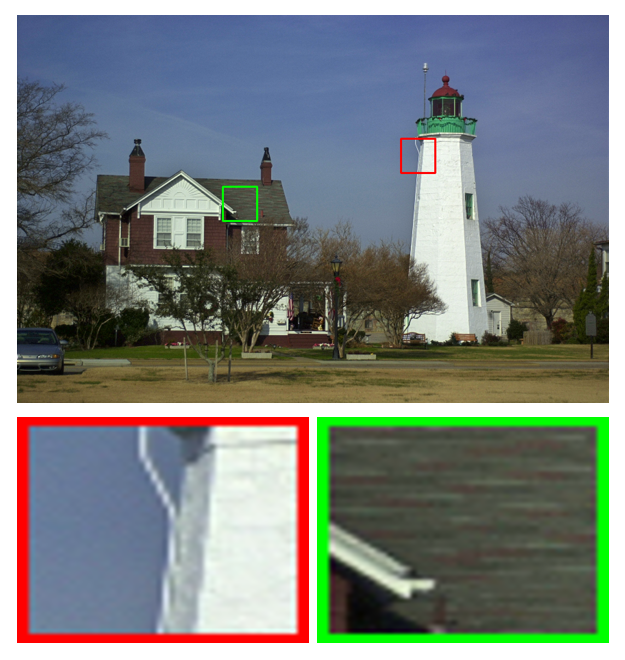
\includegraphics[width=60mm, height=48mm]{images/experiment/qualitative/comp1/prop.eps}
	\subcaption{Ours} \label{fig:qualitative/1/prop}
	\end{minipage}
	\caption{Comparison of low-light image enhancement results for test image $\#6$.}
	\label{fig:qualitative/1}
\end{figure*}
%----定性評価2の図---- %
\begin{figure*}[htbp]
\centering
	\begin{minipage}[b]{0.49\hsize}
		\centering
		\includegraphics[width=64mm, height=48mm]{images/experiment/qualitative/comp2/input.eps}
		\subcaption{Low-lgiht Image} \label{fig:qualitative/2/input}
	\end{minipage}
	\begin{minipage}[b]{0.49\hsize}
		\centering
		\includegraphics[width=64mm, height=48mm]{images/experiment/qualitative/comp2/srie.eps}
		\subcaption{SRIE} \label{fig:qualitative/2/srie}
	\end{minipage} \\
	\begin{minipage}[b]{0.49\hsize}
		\centering
		\includegraphics[width=64mm, height=48mm]{images/experiment/qualitative/comp2/wvm.eps}
		\subcaption{WVM} \label{fig:qualitative/2/wvm}
	\end{minipage}
	\begin{minipage}[b]{0.49\hsize}
		\centering
		\includegraphics[width=64mm, height=48mm]{images/experiment/qualitative/comp2/rrm.eps}
		\subcaption{RRM} \label{fig:qualitative/2/rrm}
	\end{minipage} \\
	\begin{minipage}[b]{0.49\hsize}
	\centering
	\includegraphics[width=64mm, height=48mm]{images/experiment/qualitative/comp2/lime.eps}
	\subcaption{LIME} \label{fig:qualitative/2/lime}
	\end{minipage}
	\begin{minipage}[b]{0.49\hsize}
	\centering
	\includegraphics[width=64mm, height=48mm]{images/experiment/qualitative/comp2/prop.eps}
	\subcaption{Ours} \label{fig:qualitative/2/prop}
	\end{minipage}
	\caption{Comparison of low-light image enhancement results for test image $\#7$.}
	\label{fig:qualitative/2}
\end{figure*}

\section{Quantitative Evaluation} \label{sec:quantitative}
The section focus on comparison with the proposed method and several state-of-the-art methods based on two quantitative evaluations: lightness order error (LOE) \cite{loe} and autoregressive-based image sharpness metric (ARISM) \cite{arism}. These evaluations are the indicators of naturalness. In addition, the smaller the score of these evaluations are, the better an enhanced image preserves naturalness of lightness.\par
\subsection{Lightness Order Error}
As pointed out in \cite{loe}, the relative order of lightness represents the light source directions and the lightness variation, since the naturalness of an enhanced image is related to the relative order of lightness in different local areas. LOE measures the lightness distortion of enhanced images as follows:
\begin{equation}
\mbox{LOE} = \frac{1}{m} \sum_{x=1}^{m}{RD(x)}, \label{eq:loe}
\end{equation}
where $m$ is the pixel number. Here $RD(x)$ is the relative order difference of the lightness between an observed image $S$ and the enhanced image $S^{'}$ for pixel $x$, defined by
\begin{equation}
RD(x) = \sum_{y=1}^{m}F(B(x), B(y)) \oplus F(B^{'}(x), B^{'}(y)), \label{eq:rd}
\end{equation}
where $\oplus$ stands for the exclusive-or operator, $B(x)$ and $B^{'}(x)$ are the bright channel at tje location $x$ of an observed image and the enhanced image, respectively. The function $F(p, q)$ returns $1$ if $q \in p$, $o$ otherwise. As suggested in \cite{lime}, down-sampling is needed to reduce the complexity of computing LOE. Therefore, when evaluating LOE, all images are down-sample to $50 \times 50$. As shown in Table \ref{tab:loe}, the proposed method outperforms the others in almost all dataset. This means that the proposed method can keep the naturalness of images well when enhancing.

%----LOEの表---- %
\begin{table}[tb]
	\begin{center} 
	\caption{Comparison of LOE for different methods}
	\begin{tabular}{c||c|c|c|c|c|c|c|c} \hline
	\bf{Method} & {$\#$1} & {$\#$2} & {$\#$3} & {$\#$4} & {$\#$5} & {$\#$6} & {$\#$7} & {$\#$8} \\ \hline \hline
	\textbf{SRIE} & \textcolor{red}{95.46} & \textcolor{red}{143.69} & 196.07 & \textcolor{blue}{97.46} & \textcolor{red}{104.42} & \textcolor{blue}{138.31} & \textcolor{blue}{163.81} & \textcolor{blue}{238.81} \\ \hline
	\textbf{WVM} & 187.96 & 256.22 & 205.57 & 160.27 & 238.03 & 197.29 & 295.98 & 480.98 \\ \hline
	\textbf{LIME} & 204.60 & 307.32 & 277.67 & 294.47 &  307.43 & 365.93 & 253.54 & 259.48 \\ \hline
	\textbf{RRM} & 169.25 & 290.83 & \textcolor{blue}{162.30} & 323.59 & 186.52 & 303.15 & 196.50 & 420.17 \\ \hline
	\textbf{JieP} & 161.45 & 229.53 & 208.39 & 159.85 & 252.05 & 157.89 & 259.07 & 410.72 \\  \hline \hline
	\textbf{Ours} & \textcolor{blue}{113.79} & \textcolor{blue}{186.40} & \textcolor{red}{95.79} & \textcolor{red}{80.65} & \textcolor{blue}{162.09} & \textcolor{red}{111.09} & \textcolor{red}{135.36} & \textcolor{red}{176.45} \\ \hline
	\end{tabular} \label{tab:loe}
	\end{center}
\end{table}

\subsection{Autoregressive-based image sharpness metric}
ARISM is a blind sharpness measure via parameter analysis of classical autoregressive (AR) image model. The measure estimates the sharpness in the parameter space by analyzing the difference of the locally estimated AR parameters. Moreover, the measure is taken into account the inevitable influence of color information on the sharpness assessment by extending YIQ-color space. Fig. \ref{fig:arism} shows the primary framework in ARISM, which is composed of all proceedings. Table. \ref{tab:arism} summarizes the result in ARISM. It can be seen that the proposed method achieves lower average performances than the others. This means that the proposed method can 

\cleardoublepage
%%%%%%%%%%%%%%%%%%%% Conclusion %%%%%%%%%%%%%%%%%%%%
\chapter{Conclusion} \label{sec:conclusion}
In this paper, we proposed a mixture $L_{2}$ - $L_{p}$ variational Retinex model with an adaptive texture map. First, we incorporated constraint terms on reflectance and illumination which further consider the characteristics of reflectance and illumination with a cost function of a minimization optimization problem. Next, we developed the adaptive texture map which is used to tune the noise reduction rate according to the brightness of an observed image. Moreover, the adaptive texture map contributes to reveal fine textures detail in the estimated reflectance. As the results, the proposed method can preserve texture details as much as possible while suppressing noise amplification and over-enhancement in the reflectance estimation, and smooth illumination as much as possible while keeping the structure information in the illumination estimation. Both qualitative and quantitative evaluations show that the proposed method can enhance low-light images more naturally than the state-of-the-art methods. In particular, in the LOE evaluation, the proposed method outperforms the other methods in almost all the images.
\cleardoublepage
%%%%%%%%%%%%%%%%%%%% Acknowledgement %%%%%%%%%%%%%%%%%%%%
\chapter*{Acknowledgement}
\label{sec:acknowledgement}
I would like to give heartfelt thanks to Prof. Youji Iiguni who provided fruitful suggestions and helpful comments and help in interpreting the significance of this study. I also appreciate to Associate Prof. Ryota Shimokura who provided helpful comments and suggestions in practical aspect. Finally, I would like to thank all the Bachelor, Master, Doctor students in Iiguni laboratory.
\cleardoublepage
%%%%%%%%%%%%%%謝辞,参考文献,付録%%%%%%%%%%%%%%
\appendix % 付録

\renewcommand{\thesection}{\Alph{section}}
\renewcommand{\thesubsection}{\thesection-\Roman{subsection}}

\makeatletter % プリアンブルで@を使うために必要
 \renewcommand{\theequation}{A.\arabic{equation}}
\makeatother % プリアンブルで@を使うために必要

\include{app}

\begin{thebibliography}{99}
\bibitem{he1} E. D. Pisano $et$ $al$, ``Contrast limited adaptive histogram equalization image processing to improve the detection of simulated speculations in dense mammograms,'' J. Digit. Image, vol. 11, no. 4, pp. 193-200, 1998.
\bibitem{he2} H, Cheng and X. Shi, ``A simple and effective histogram equalization approach to image enhancement,'' Digital Signal Processing, vol. 14, no. 2, pp. 158-170, 2004.
\bibitem{he3} S.-C. Huang, F.-C. Cheng, and Y.-S. Chiu, ``Efficient contrast enhancement using adaptive gama correction with weighting distribution,'' IEEE Trans. Image Process., vol. 20, no. 5, pp. 1262-1272, 2011.
\bibitem{haze1} L. Li, R. Wang, W. Wamg, and W. Gao, ``A low-light image enhancement method for both denoising and contrast enlarging,'' in Proc. IEEE Int. Conf. Image Process., pp. 3730-3734, 2015.
\bibitem{haze2} X.Zhang, P.Shen, L. Luo, L. Zhang, and J. Song, ``Enhancement and noise reduction of very low light level images,'' in Proc. 21st Int. Conf. Pattern Recognit. (ICPR), pp. 2034-2037, 2012. 
\bibitem{ssr} D. J. Jobson, Z.-U. Rahman, and G. A. Woodell, ``Properties and performance of a center/surround retinex,'' IEEE Trans. Image Process., vol. 6, no. 3, pp. 451-462, 1997.
\bibitem{msr} D. J. Jobson, Z.-U. Rahman, and G. A. Woodell, ``A multiscale retinex for briding the gap between color images and the human observation of scenes,'' IEEE Trans. Image Process, vol. 6, no. 7, pp. 965-976, 1997.
\bibitem{srie}X. Fu, Y. Liao, D. Zeng, Y. Huang, X. Zhang, and X. Ding, ``A probabilistic method for image enhancement with simultaneous illumination and reflectance estimation,'' IEEE Trans. Image Process., vol. 24, no. 12, pp. 4965-4977, 2015.
\bibitem{wvm}X. Fu, D. Zeng, Y. Huang, X. Zhang and X. Ding, ``A weighted variational model for simultaneous reflectance and illumination estimation, '' IEEE Conf. Computer Vis. Pattern Recognit., pp. 2782-2790, 2016.
\bibitem{lime} X. Guo, Y. Li, and H. Ling, ``LIME: Low-light image enhancement via illumination map estimation,'' IEEE Trans. Image Process., vol. 26, no. 2, pp. 982-993, 2017. 
\bibitem{jiep} B. Cai, X. Xu, K. Guo, K. Jia, B. Hu, and D. Tao, ``A joint intrinsic-extrinsic prior model for retinex,'' In Proc., IEEE Conf. Computer Vis., Pattern Recognit., pp. 4000-4009, 2017.
\bibitem{rrm} M. Li, J. Liu, W. Yang, X. Sun, and Z. Guo, ``Structure-revealing low-light image enhancement via robust Retinex model, '' IEEE Trans. Image Process., vol. 27, no. 6, pp. 2828-2841, 2018.
\bibitem{retinex} E. H. Land and J. J. McCann, ``Lightness and retinex theory,'' J. Opt. Soc. Amer., vol. 61, no. 1, pp. 1-11, 1971.
\bibitem{guided} K. He, J. Sun, and X. Tand, ``Guided image filtering,'' Proc. European Conf. on Computer Vis., pp. 1-14, 2010.
\bibitem{l2-lp} C. Fu, L. Duan, and C. Xiao, ``A hybrid L2-Lp variational model for single low-light image enhancement with bright channel prior,'' IEEE Int. Conf. on Image Process. (ICIP), 2019.
\bibitem{arpr} N. Bonneel, B. Kovacs, S. Paris, and K. Bala, ``Intrinsic decompositions for image editing,'' Computer Graphics Forum, vol.36, no. 2, 2017.
\bibitem{block} P. Tseng, ``Convergence of a block coordinate descent method for nondifferentiable minimization,'' Journal of Optimization Theory and Applications, vol. 109, no. 3, pp. 475-494, 2001.
\bibitem{iterate} E. J. Candes, M. B. Wakin, and S. P. Boyd, ``Enhancing sparsity by reweighted $l_{1}$ minimization,'' Journal of Fourier Analysis and Applications, vol. 14, no. 5-6, pp. 877-905, 2008. 
\bibitem{l0-sparse} L. Xu, S.Zheng, and J. Jia, ``Unnatural l0 sparse representation for natural image debluring,'' IEEE Conf. Computer Vis. Pattern Recognit., pp. 1107-1114, 2013.
\bibitem{bright} X. Fu, D. Zheng, Y. Huang, X. Ding, and X-P. Zhang, ``A variational framework for single low light image enhancement using bright channel prior, '' in Proc. IEEE Global Conf. on Signal and Inform. Process., pp. 1085-1088, 2013.
\bibitem{activation} S. Park, S. Yu, B. Moon, S. Ko, and J. Paik, ``Low-light image enhancement using variational optimization-based retinex model,'' IEEE Trans. on Cons. Elec., vol. 63, no. 2, pp. 178-184, 2017.
\bibitem{loe} S. Wang, J. Zheng, H.-M. Hu, and B. Li, ``Naturalness preserved enhancement algorithm for non-uniform illumination images,'' IEEE Trans. Image Process., vol. 22, no. 9, pp. 3538-3578, 2013.
\bibitem{arism} K. Gu, G. Zhai, W. Lin, X. Yang, and W. Zhang, ``No reference image sharpness assessment in autoregressive parameter space,'' IEEE Trans. on Image Process., vol. 24, no. 10, pp. 3218-3231, 2015.
\end{thebibliography}
\chapter*{Publication}
\label{sec:BIO}

\section*{International Conference}
\begin{itemize}
\item
Kazuki Kurihara, Hiromi Yoshida, and Youji Iiguni, 
 "Low-Light Image Enhancement via Adaptive Shape and Texture Prior",
 Proc. of 15th International Conference on Signal Image Technology $\&$ Internet Based Systems (SITIS 2019), pp. 74-81, Nov. 2019. 
\end{itemize}

\section*{Domestic Conference}
\begin{itemize}
\item
栗原 一樹, 吉田 大海, 飯國洋二,
"Variational Retinex Modelと活性化マップを用いた夜間低照度画像の鮮明化",
画像電子学会 第286回研究会, Aug. 2018.
\end{itemize}
%%%%%%%%%%%%%%%%%%%%%%%%%%%%%%%%%%%%%%%%%%%%%%

\end{document}
